\documentclass[11pt]{article}

%%%%%%%%%%%%
% Packages %
%%%%%%%%%%%%
\usepackage[dvipsnames]{xcolor}
\hyphenpenalty=10000
\usepackage{tikz}
\usetikzlibrary{shapes,arrows}

\usepackage{tocloft}
\renewcommand\cftsecleader{\cftdotfill{\cftdotsep}}
\def\undertilde#1{\mathord{\vtop{\ialign{##\crcr
$\hfil\displaystyle{#1}\hfil$\crcr\noalign{\kern1.5pt\nointerlineskip}
$\hfil\tilde{}\hfil$\crcr\noalign{\kern1.5pt}}}}}
\usepackage{cleveref}
\usepackage{xcolor}
\usepackage[colorlinks = true,
            linkcolor = black,
            urlcolor  = black,
            citecolor = black,
            anchorcolor = black]{hyperref}
\usepackage{epstopdf}
\usepackage{braket}
\usepackage{upgreek}
\usepackage{caption}
\usepackage{booktabs}
\usepackage{subcaption}
\usepackage{amssymb,latexsym,amsmath,gensymb}
\usepackage{latexsym}
\usepackage{graphicx}
\usepackage{float}
\usepackage{enumitem}
\usepackage{pdflscape}
\usepackage{url}
\usepackage{array}
\newcolumntype{C}{>{$\displaystyle} c <{$}}
\usepackage{tikz, calc}
\usetikzlibrary{shapes.geometric, arrows, calc}
\tikzstyle{norm} = [rectangle, rounded corners, minimum width=2cm, minimum height=1cm,text centered, draw=black]
\tikzstyle{arrow} = [thick, ->, >=stealth]

\newcommand{\argmin}{\arg\!\min}
\newcommand{\me}{\mathrm{e}}
\providecommand{\e}[1]{\ensuremath{\times 10^{#1}}} 
\providecommand{\mb}[1]{\mathbf{#1}}
\providecommand{\mf}[1]{\mathbf{#1}}
\providecommand{\ro}[1]{\mathbf{\mathbf{r}}_o}
\providecommand{\so}[1]{\mathbf{\hat{s}}_o}
\providecommand{\rb}[1]{\mathbf{r}_b}
\providecommand{\rbm}[1]{r_b^{\text{m}}}
\providecommand{\rd}[1]{\mathbf{r}_d}
\providecommand{\mh}[1]{\mathbf{\hat{#1}}}
\providecommand{\bs}[1]{\boldsymbol{#1}} 
\providecommand{\intinf}{\int_{-\infty}^{\infty}}
\providecommand{\fig}[4]{
  % filename, width, caption, label
\begin{figure}[h]
 \captionsetup{width=1.0\linewidth}
 \centering
 \includegraphics[width = #2\textwidth]{#1}
 \caption{#3}
 \label{fig:#4}
\end{figure}
}

\newcommand{\tensor}[1]{\overset{\text{\tiny$\leftrightarrow$}}{\mb{#1}}}
\newcommand{\tunderbrace}[2]{\underbrace{#1}_{\textstyle#2}}
\providecommand{\figs}[7]{
  % filename1, filename2, caption1, caption2, label1, label2, shift
\begin{figure}[H]
\centering
\begin{minipage}[b]{.45\textwidth}
  \centering
  \includegraphics[width=1.0\linewidth]{#1}
  \captionsetup{justification=justified, singlelinecheck=true}
  \caption{#3}
  \label{fig:#5}
\end{minipage}
\hspace{2em}
\begin{minipage}[b]{.45\textwidth}
  \centering
  \includegraphics[width=1.0\linewidth]{#2}
  \vspace{#7em}
  \captionsetup{justification=justified}
  \caption{#4}
  \label{fig:#6}
\end{minipage}
\end{figure}
}
\makeatletter

\providecommand{\code}[1]{
\begin{center}
\lstinputlisting{#1}
\end{center}
}

\newcommand{\crefrangeconjunction}{--}
%%%%%%%%%%%
% Spacing %
%%%%%%%%%%%
% Margins
\usepackage[
top    = 1.5cm,
bottom = 1.5cm,
left   = 1.5cm,
right  = 1.5cm]{geometry}

% Indents, paragraph space
%\usepackage{parskip}
\setlength{\parskip}{1.5ex}

% Section spacing
\usepackage{titlesec}
\titlespacing*{\title}
{0pt}{0ex}{0ex}
\titlespacing*{\section}
{0pt}{0ex}{0ex}
\titlespacing*{\subsection}
{0pt}{0ex}{0ex}
\titlespacing*{\subsubsection}
{0pt}{0ex}{0ex}

% Line spacing
\linespread{1.1}

%%%%%%%%%%%%
% Document %
%%%%%%%%%%%%
\begin{document}
\title{\vspace{-2.5em} Spatio-angular transfer functions for fluorescence microscopes\vspace{-1em}}  \author{Talon Chandler, Min Guo, Hari Shroff, Rudolf Oldenbourg, Patrick La Rivi\`ere}
\date{\vspace{-1em}\today\vspace{-1em}}
\maketitle
\begin{abstract}
  We investigate how the orientation and position of fluorescent dipole emitters
  affects microscopic imaging using electromagnetic optics theory. Starting with
  the thoroughly studied spatio-angular point spread function, we introduce the
  spatio-angular coherent spread function, coherent transfer function, and
  optical transfer function as electromagnetic extensions of well-known
  functions in scalar optics theory. We use these concepts to show that
  fluorescence microscopes have a spatio-angular band limit. 
\end{abstract}
\section{Introduction}

We use plain roman type for scalars, e.g., $x, y, z$; bold lowercase roman type
for two-dimensional vectors, e.g., $\mb{r}$; hats for unit vectors, e.g.,
$\mb{\hat{s}}$; and bold capital roman type for matrices, e.g.,
$\mb{R}$. We use the real spherical harmonic functions
\begin{align}
  y_l^m(\vartheta, \varphi) =
  \begin{cases}
    \sqrt{2}K_l^m\cos(m\varphi)P_l^m(\cos\vartheta), & m > 0\\
    K_l^0P_l^0(\cos\vartheta), & m = 0\\
    \sqrt{2}K_l^m\sin(-m\varphi)P_l^{-m}(\cos\vartheta), & m < 0\\
  \end{cases}
\end{align}
where
\begin{align}
  K_l^m = \sqrt{\frac{(2l+1)}{4\pi}\frac{(l-|m|)!}{(l+|m|)!}},
\end{align}
and $P_l^m(x)$ are the associated Legendre polynomials. The $l=0$ and $l=1$
spherical harmonics are given by
\begin{equation}
\begin{aligned}
  y_0^0(\vartheta, \varphi) &= \sqrt{\frac{1}{4\pi}},\\
  y_1^{-1}(\vartheta, \varphi) = \sqrt{\frac{3}{4\pi}}\sin\varphi\sin\vartheta, \hspace{2em} y_1^0(\vartheta, \varphi) &= \sqrt{\frac{3}{4\pi}}\cos\vartheta, \hspace{2em} y_1^1(\vartheta, \varphi) = \sqrt{\frac{3}{4\pi}}\cos\varphi\sin\vartheta. \label{eq:harmonics}
\end{aligned}
\end{equation}

\section{Spatio-angular point spread functions}
\begin{figure}[h]
 \captionsetup{width=1.0\linewidth}
 \centering
   \centering
   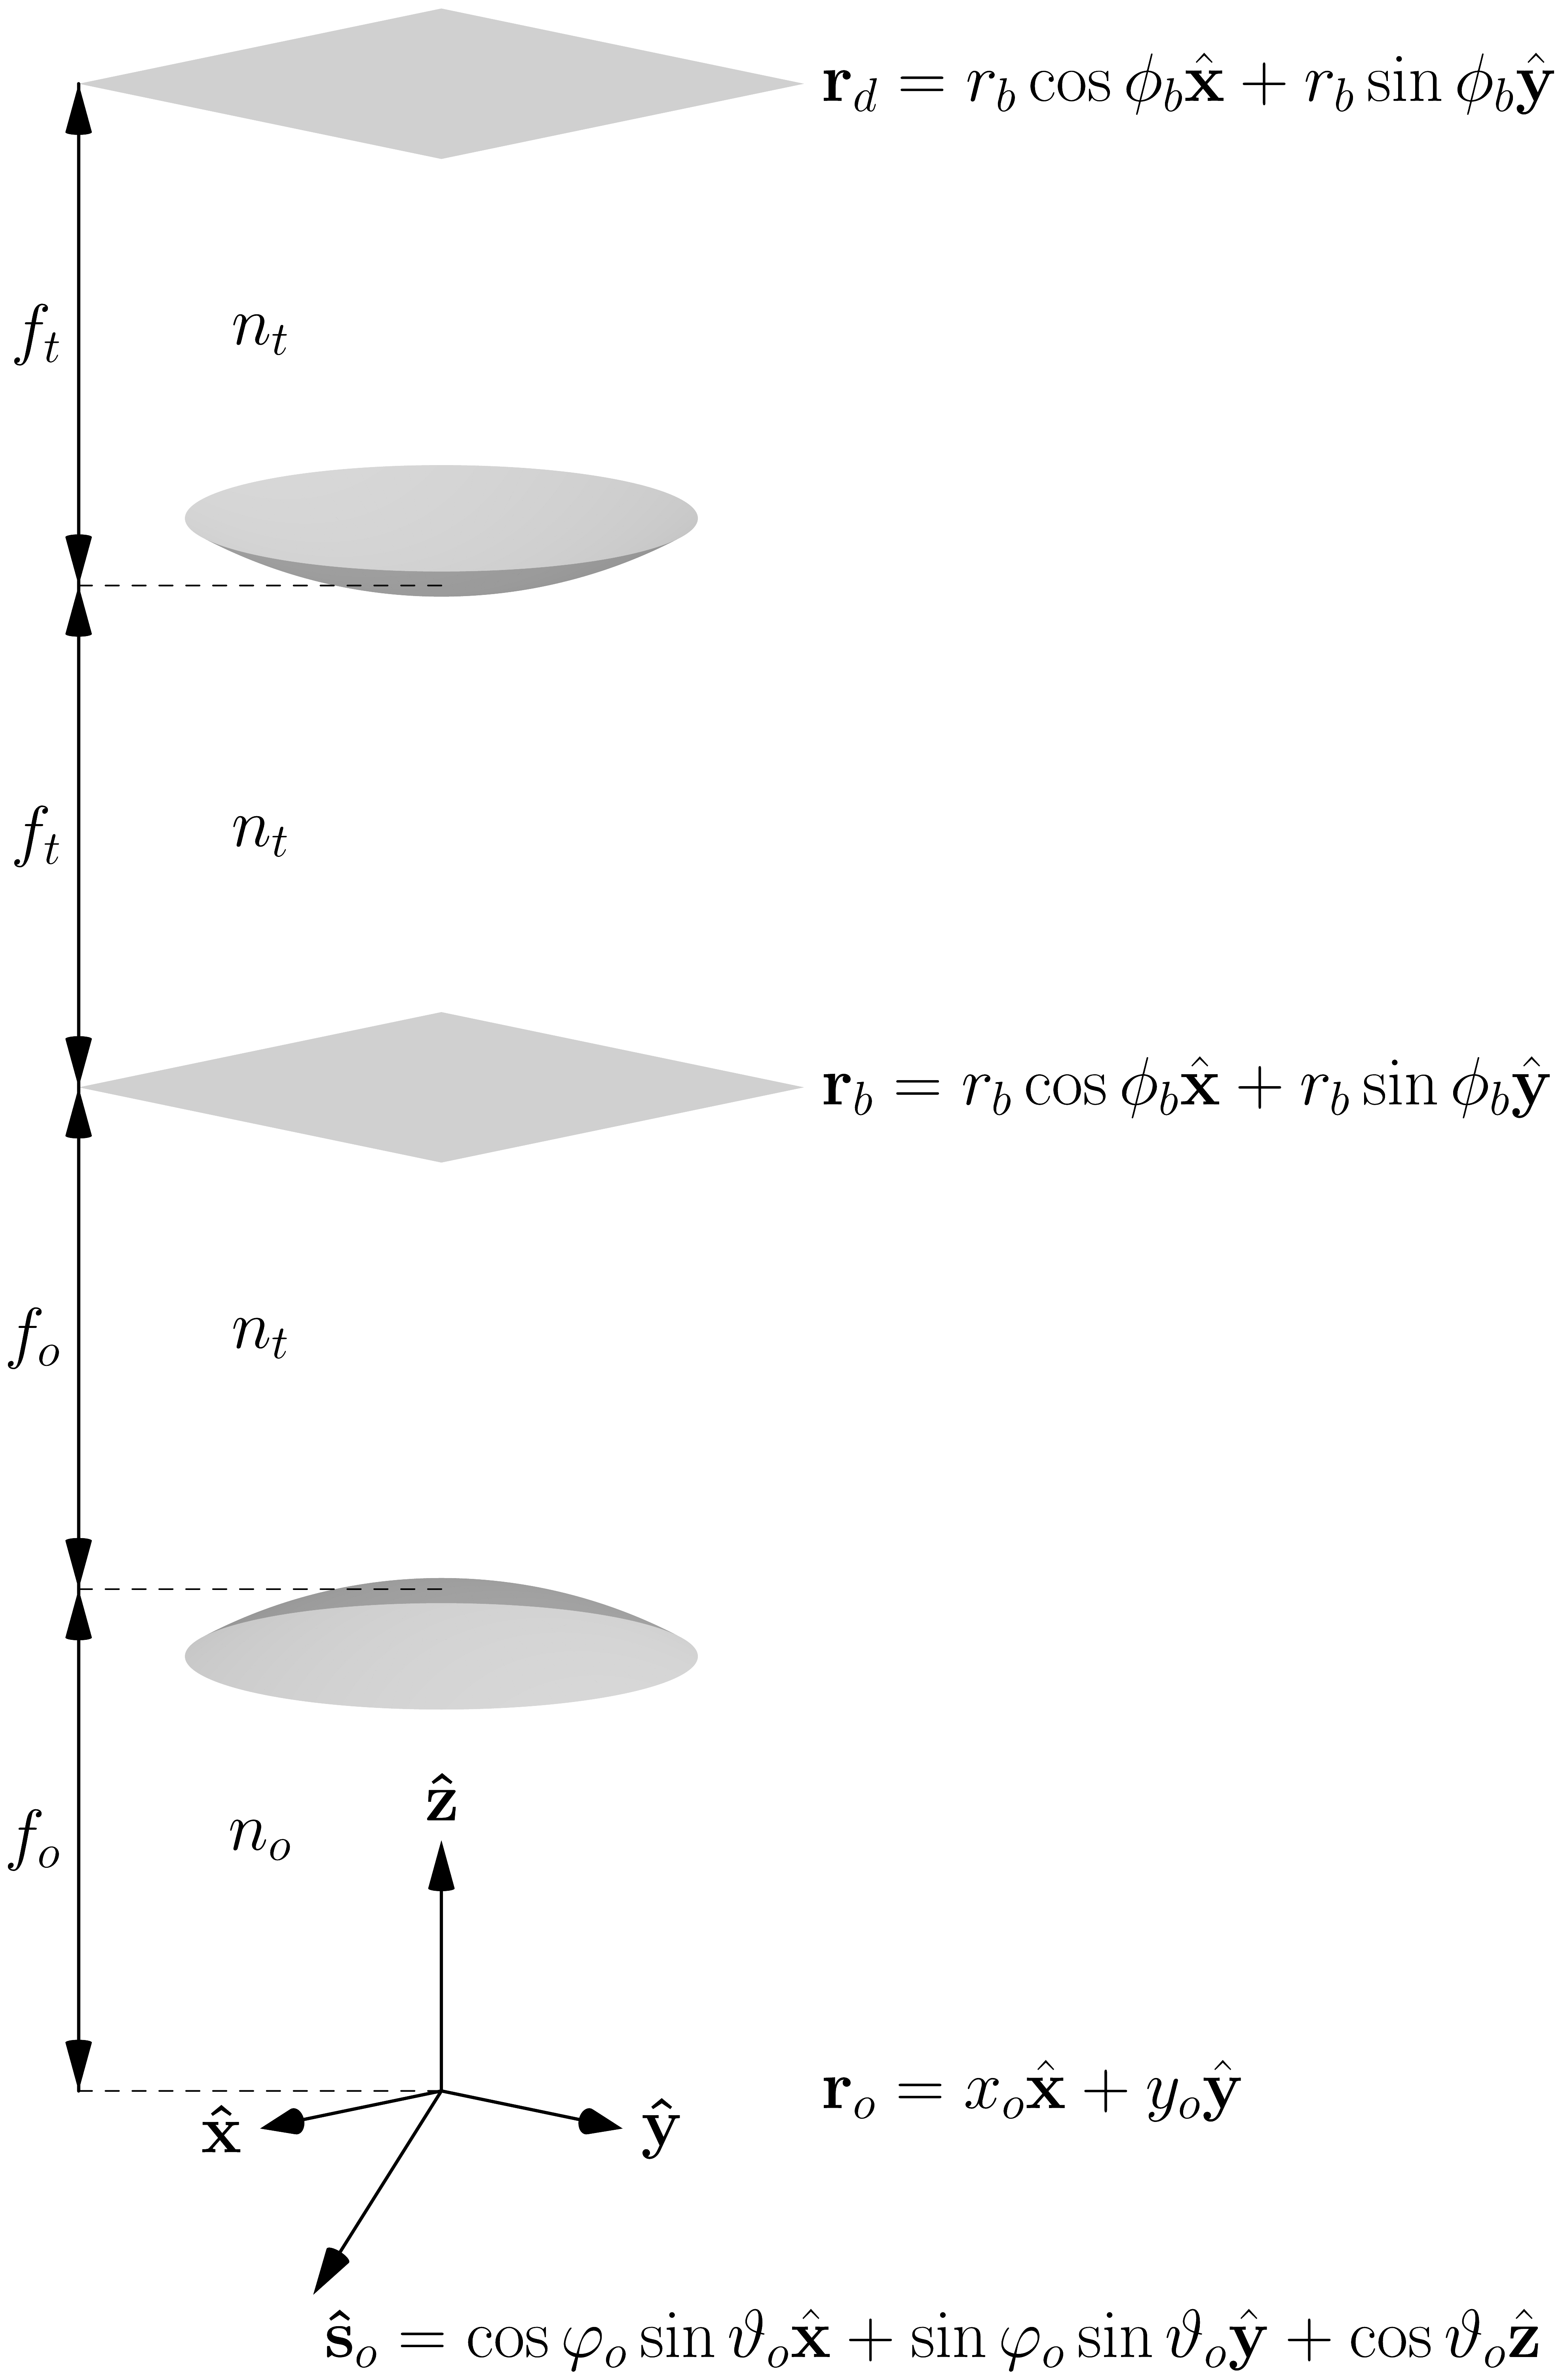
\includegraphics[width = 0.4\textwidth]{../figures/schematic.pdf}
   \caption{Simplified schematic of a single-view fluorescence microscope. The
     object is placed near the focal point of an aplanatic objective lens with
     focal length $f_{o}$ in a medium with refractive index $n_o$. The object is
     parameterized by the 2D position vector $\ro{}$ ($o$ for object) and an
     orientation unit vector $\so{}$. The light emitted by the fluorescent
     object is collected and collimated by the objective lens so that the
     electric fields are purely transverse in the back focal plane. Points in
     the back focal plane are parameterized by a 2D position vector $\rb{}$ ($b$
     for back focal plane). Finally, the tube lens with focal length $f_t$
     refocuses the light onto a detector. Points on the detector are
     parameterized by a 2D position vector $\rd{}$ ($d$ for detector). The back
     focal plane and detector are in a medium with refractive index $n_t$. Note
     that this schematic is not to scale---we consider the case where
     $f_o \ll f_t$.}
   \label{fig:frames_a}
\end{figure}

Figure \ref{fig:frames_a} shows a schematic of the fluorescence microscope that
we are considering with a summary of our notation. We start by following Backer
and Moerner \cite{backer2014} to find the electric field at position $\rb{}$ in
the back focal plane due to a single dipole emitter at position $\ro{}$ oriented
along $\so{}$ as
\begin{align}
  \mb{\tilde{e}}_b(\rb{};\ro{}, \so{}) \propto \me^{-i(kn_o/f_o)\rb{}\cdot\ro{}}\sqrt{\frac{1}{\rho_b}}
  \begin{bmatrix}
    \sin^2\phi_b + \rho_b\cos^2\phi_b&\sin\phi_b\cos\phi_b(\rho_b - 1)&-\frac{r_b}{f_o}\cos\phi_b\\
    \sin\phi_b\cos\phi_b(\rho_b - 1)&\cos^2\phi_b + \rho_b\sin^2\phi_b&-\frac{r_b}{f_o}\sin\phi_b\\
    0&0&0
  \end{bmatrix}
  \begin{bmatrix}
    \cos\varphi_o\sin\vartheta_o\\
    \sin\varphi_o\sin\vartheta_o\\
    \cos\vartheta_o
  \end{bmatrix}
\Pi\left(\frac{r_b}{r_b^{\text{max}}}\right)\label{eq:bfp},
\end{align}
where we define $\rho_b \equiv \sqrt{1 - \left(\frac{r_b}{f_o}\right)^2}$, and
$\Pi(x)$ is a boxcar function that returns 1 when $|x| < 1$ and 0 otherwise. We
can understand this expression term by term---the exponential term accounts for
the phase as dipole emitter is moved in object space, the square root term
conserves power before and after the objective lens, the matrix models the
dipole emission process and electric field rotation caused by the objective
lens, the vector is the dipole orientation unit vector, and
$\Pi\left(\frac{r_b}{r_b^{\text{max}}}\right)$ accounts for the numerical
aperture of the lens with $r_b^{\text{max}} = \frac{f_0}{n_0}\text{NA}$. We use
a tilde to mark single dipole response functions---we will consider the response
due to a field of dipoles in the next section.

Although we will not use the result immediately, we can write the electric field
in the back focal plane under the paraxial approximation. We expand Eq. \ref{eq:bfp}
in a Taylor series about $r_b=0$ and drop all second-order and higher terms to
find
\begin{align}
  \mb{\tilde{e}}^{(p)}_b(\rb{};\ro{}, \so{}) \propto \me^{-i(kn_o/f_o)\rb{}\cdot\ro{}}
  \begin{bmatrix}
    1 & 0 &-\frac{2r_b}{f_o}\cos\phi_b\\
    0&1&-\frac{2r_b}{f_o}\sin\phi_b\\
    0&0&0
  \end{bmatrix}
  \begin{bmatrix}
    \cos\varphi_o\sin\vartheta_o\\
    \sin\varphi_o\sin\vartheta_o\\
    \cos\vartheta_o
  \end{bmatrix}
\Pi\left(\frac{r_b}{r_b^{\text{max}}}\right).\label{eq:bfppara}
\end{align}
We will continue to use a superscript $(p)$ to mark terms that have used the
paraxial approximation.

If the tube lens is weakly focusing ($f_o \ll f_t$) then we can find the
electric field in the detector plane by taking the Fourier transform of the
electric field in the back focal plane
\begin{align}
  \mb{\tilde{e}}_d(\rd{}; \ro{}, \so{}) \propto \int_{\mathbb{R}^2} d\rb{}\, \tilde{\mb{e}}_b(\rb{}; \ro{}, \so{})\me^{-i (kn_t/f_t) \rb{} \cdot \rd{}}. \label{eq:ed}
\end{align}
By isolating the phase term in Eq. \ref{eq:bfp} with
$\mb{\tilde{e}}_b(\rb{};\ro{}, \so{}) \equiv \me^{-i(kn_o/f_o)\rb{}\cdot\ro{}}
\tilde{\underline{\mb{e}}}_b(\rb{};\so{})$, and plugging into Eq. \ref{eq:ed} we find
that 
\begin{align}
  \mb{\tilde{e}}_d(\rd{} - M\ro{}, \so{}) \propto \int_{\mathbb{R}^2} d\rb{}\, \tilde{\underline{\mb{e}}}_b(\rb{}; \so{})\me^{-i (kn_t/f_t)\, \rb{} \cdot [\,\rd{} - M\ro{}]}.
\end{align}
where $M = -\frac{n_o}{n_t}\frac{f_t}{f_o}$ is the transverse magnification.  By
writing the electric field in the detector plane in terms of $\rd{} - M\ro{}$,
we have established that the electric field in the detector plane is
\textit{transverse shift-invariant}---a transverse shift of the object creates a
magnified transverse shift of the image. We define coordinates on the detector
centered on the image of the object
$\rd{}' \equiv \rd{} - M\ro{} = r_d'\cos\phi_d'\mh{x} + r_d'\sin\phi_d'\mh{y}$,
then we follow Novotny \cite{nov2006} by writing the integrals in polar
coordinates, evaluating the azimuthal integrals, and writing the result
concisely in terms of three radial integrals
\begin{align}
  \tilde{\mb{e}}_d(\rd{}', \so{}) &\propto
  \begin{bmatrix}
    a(r_d') + c(r_d')\cos(2\phi_d') & c(r_d')\sin(2\phi_d') & 2ib(r_d')\cos\phi_d'\\
    c(r_d')\sin(2\phi_d') & a(r_d') - c(r_d')\cos(2\phi_d') & 2ib(r_d')\sin\phi_d'\\
    0&0&0\\
  \end{bmatrix}
  \begin{bmatrix}
    \cos\varphi_o\sin\vartheta_o\\
    \sin\varphi_o\sin\vartheta_o\\
    \cos\vartheta_o
  \end{bmatrix},\label{eq:elec}
\end{align}
where $a(r_d'), b(r_d')$, and $c(r_d')$ are
\begin{align}
  a(r_d') &= \int_0^{\theta_{\text{max}}}d\theta\ \sqrt{\cos\theta}\sin\theta(1+\cos\theta)J_0(k_b r_d'\sin\theta f_o/f_t),\\%\ \text{exp}\left\{ik_bz_o[1-(1/2)(f_o/f_t)^2\sin^2\theta]\right\},\\
  b(r_d') &= \int_0^{\theta_{\text{max}}}d\theta\ \sqrt{\cos\theta}\sin^2\theta J_1(k_b r_d'\sin\theta f_o/f_t),\\%\ \text{exp}\left\{ik_bz_o[1-(1/2)(f_o/f_t)^2\sin^2\theta]\right\},\\
  c(r_d') &= \int_0^{\theta_{\text{max}}}d\theta\ \sqrt{\cos\theta}\sin\theta(1-\cos\theta)J_2(k_b r_d'\sin\theta f_o/f_t).%\ \text{exp}\left\{ik_bz_o[1-(1/2)(f_o/f_t)^2\sin^2\theta]\right\}.
\end{align}
We can identify Eq. \ref{eq:elec} as the vector-valued \textit{coherent spread
  function} (CSF) of the microscope. The more familiar scalar-valued
CSF---sometimes called the amplitude transfer function---is only applicable to
cases where electromagnetic optics plays no role in the microscope---not true
for samples that contain dipole emitters.

To build our intuition about the CSF, we will rewrite the matrix multiplication
in Eq. \ref{eq:elec} in terms of the spherical harmonics. Notice that the $l=1$
spherical harmonics are the Cartesian components of the unit dipole axis (see
Eq. \ref{eq:harmonics}), so the CSF becomes
\begin{align}
  \tilde{\mb{e}}_d(\rd{}', \so{}) &\propto
  \begin{bmatrix}
    [a(r_d') + c(r_d')\cos(2\phi_d')]y_1^{1}(\so{}) + c(r_d')\sin(2\phi_d')y_1^{-1}(\so{}) + 2ib(r_d')\cos\phi_d'y_1^{0}(\so{})\\
    c(r_d')\sin(2\phi_d')y_1^{1}(\so{}) + [a(r_d') - c(r_d')\cos(2\phi_d')]y_1^{-1}(\so{}) + 2ib(r_d')\sin\phi_d'y_1^{0}(\so{})\\
    0\\
  \end{bmatrix}.
\end{align}
By applying the paraxial approximation ($\sin\theta\approx\theta$ and
$\cos\theta\approx 1$), the integrals $a(r_d'), b(r_d')$ and $c(r_d')$ can be
evaluated in terms of Bessel functions. We can evaluate $a(r_d')$ and $b(r_d')$ with the
help of $\int_0^zdx\ xJ_0(ax) = zJ_1(az)/a$ and
$\int_0^zdx\ x^2J_1(ax) = z^2J_2(az)/a$, respectively, and $c(r_d') = 0$ because
$J_2(x)$ is zero to first order. In this case, the CSF simplifies to
\begin{align}
  \tilde{\mb{e}}^{(p)}_d(\rd{}', \so{}) &\propto
  \begin{bmatrix}
    a^{(p)}(r_d')y_1^{1}(\so{}) + 2ib^{(p)}(r_d')\cos\phi_d'y_1^{0}(\so{})\\
    a^{(p)}(r_d')y_1^{-1}(\so{}) + 2ib^{(p)}(r_d')\sin\phi_d'y_1^{0}(\so{})\\
    0\\
  \end{bmatrix}\label{eq:paracsf},
\end{align}
where the integrals evaluate to
\begin{align}
  {a^{(p)}}(r_d') = \frac{J_1(2\pi \nu_or_d')}{\pi \nu_or_d'}, 
  &\hspace{2em}
    {b^{(p)}}(r_d') = \frac{\text{NA}}{n_o}\left[\frac{J_2(2\pi \nu_or_d')}{\pi \nu_or_d'}\right],  \label{eq:abparadef}
  \intertext{and we have substituted}
  \nu_o \equiv \frac{\text{NA}}{M\lambda},&\hspace{2em}
  \text{NA} \equiv n_o\sin\theta_{\text{max}}.
\end{align}
Under the paraxial approximation the electric fields on the detector created by
a single dipole are composed of two parts, a parallel part and a radial
part. The coefficients of the $y_1^0$ spherical harmonic in Eq. \ref{eq:paracsf}
create the radial part of the field---the $z$ component of the dipole generates
a radial field on the detector with respect to the image point. The coefficients
of the $y_1^1$ and $y_1^{-1}$ spherical harmonics create a parallel field in the
detector plane parallel to the $x$ and $y$ components of the
dipole. As the NA increases and the paraxial approximation no longer applies, we
begin to see coupling between the $x$ and $y$ components of the dipole with the $y$ and $x$ transverse fields, respectively.

We can find the intensity in the detector plane due to a single dipole
by taking the squared modulus of the CSF
\begin{align}
  h(\rd{}', \so{}) = \left|\tilde{\mb{e}}_d(\rd{}', \so{})\right|^2 \label{eq:kernel}.
\end{align}
For convenience we keep the CSF written in terms of the spherical harmonics and
use a table of spherical harmonic products (see Appendix \ref{realspherical}) to
calculate the intensity in the detector plane as
\begin{equation}
  \begin{split}
  h(\rd{}', \so{}) \propto &\left(a^2(r_d') + 2b^2(r_d') + c^2(r_d')\right)y_0^0(\so{}) -\frac{2\sqrt{15}}{5}a(r_d')c(r_d')\sin(2\phi_d')y_2^{-2}(\so{})\\ &+ \frac{1}{\sqrt{5}}\left(-a^2(r_d') + 4b^2(r_d') - c^2(r_d')\right)y_2^{0}(\so{}) +\frac{2\sqrt{15}}{5}a(r_d')c(r_d')\cos(2\phi_d')y_2^{2}(\so{}). \label{eq:kerna}
\end{split}
\end{equation}
We can identify Eq. \ref{eq:kerna} as the spatio-angular \textit{point spread
  function} (PSF) of the microscope. Writing the spatio-angular PSF in terms of
spherical harmonic functions has two advantages. First, it allows us to express
the spatio-angular PSF very concisely. Instead of considering the point spread
function for every possible dipole orientation, we only need to consider four
spatio-angular PSFs---one for each spherical harmonic. Second, the spherical
harmonic functions form an orthonormal basis for functions on the sphere---a
convenient fact that we will use later.

It is useful to compare Eq. \ref{eq:kerna} to Backer and Moerner's approach
\cite{backer2014}. They expand the spatio-angular PSF in terms of six second
moments of the fluorophore distribution
$\{s_x^2, s_y^2, s_z^2, s_xs_y, s_xs_z, s_ys_z\}$. This approach is very
useful---only six precomputed spatio-angular PSFs are required to represent an
arbitrary spatio-angular PSF. Instead of expanding in terms of six second
moments, we expand onto just four spherical harmonics which, unlike the second
moments, are orthonormal functions. In the next section we will use the
orthonormality of the spherical harmonics to derive spatio-angular transfer
functions for fluorescence microscopes.

The spatio-angular PSF under the paraxial approximation is given by
\begin{align}
      h^{(p)}(\rd{}', \so{}) \propto \left({a^{(p)}}^2(r_d') + 2{b^{(p)}}^2(r_d')\right)y_0^0(\so{}) + \frac{1}{\sqrt{5}}\left(-{a^{(p)}}^2(r_d') + {4b^{(p)}}^2(r_d')\right)y_2^{0}(\so{})\label{eq:para}.
\end{align}
We rewrite the PSF in the following form to make plotting and interpretation easier
\begin{align}
  h^{(p)}(\rd{}', \so{}) &= {h_0^0}^{(p)}(\rd{}')y_0^0(\so{}) + {h_2^0}^{(p)}(\rd{}')y_2^0(\so{}),\\
  {h_0^0}^{(p)}(\rd{}') &\equiv {a^{(p)}}^2(r_d') + 2{b^{(p)}}^2(r_d'),\\
  {h_2^0}^{(p)}(\rd{}') &\equiv \frac{1}{\sqrt{5}}\left[- {a^{(p)}}^2(r_d') + 4{b^{(p)}}^2(r_d')\right]. \label{eq:concisepsf}
\end{align}

First, consider the coefficient on the $y_0^0$ spherical harmonic in Eq.
\ref{eq:para}. This coefficient is the point spread function for an angularly
uniform distribution of fluorophores. The first term of the coefficient
${A^{(p)}}^2(r_d')$ is the familiar Airy disk that arises from the contribution
of dipoles oriented in the transverse plane, while the second term
${B^{(p)}}^2(r_d')$ is a smaller factor that arises from dipoles oriented
outside of the transverse plane. This leads to an interesting conclusion---a
uniform distribution of dipoles has a point spread function that is slightly
wider than an Airy disk even in the paraxial approximation. The Airy disk is
usually derived using paraxial scalar optics while here we have used paraxial
electromagnetic optics. Therefore, we can consider the second term to be an
electromagnetic correction to the Airy disk. We will quantify this difference in
the next section.

Next, consider the coefficient on the $y_2^0$ spherical harmonic in
Eq. \ref{eq:para}. This coefficient is the spatial PSF for a distribution of
fluorophores proportional to $3\cos^2\vartheta_o - 1$. Counterintuitively, this
fluorophore distribution cannot exist because it would require a negative number
of fluorophores along some orientations; but if this distribution could exist,
then this coefficient would be its spatial PSF. Considering negative
distributions of fluorophores in our calculations should not be cause for
concern. The spherical harmonics span the space of functions on the sphere, so
any positive fluorophore distribution can be represented by the spherical
harmonics and we never need to consider negative fluorophores.
    
Finally, consider all of the spherical harmonics that have a zero
coefficient. These spherical harmonics span the angular null space of our
measurement system---fluorophore distributions that lie in the null space do not
affect the measured intensities. Under the paraxial approximation all of the
non-zero coefficients are rotationally symmetric ($m=0$) spherical harmonics,
which means that the transverse orientation of the dipoles does not affect the
PSF. In the high NA case this is no longer true---two $m=2$ spherical harmonics
have non-zero coefficients and the transverse orientation of dipoles does affect
the PSF.


\section{Spatio-angular transfer functions}
Consider a thin object that consists of fluorescent dipoles in arbitrary
positions and orientations. We can represent the entire object using a function
$\bs{\mu}(\ro{}, \so{})$ that returns a complex-valued vector for each position
$\ro{}$ and direction $\so{}$. The magnitude of the complex-valued vector is the
magnitude of the dipole moment and the elements of the vector give the orientation
and phase of the radiating dipole moment. Because $\bs{\mu}(\ro{}, \so{})$
includes the relative phases of different points and orientations in the object,
$\bs{\mu}(\ro{}, \so{})$ can represent coupled dipoles that are emitting
partially or completely coherently.

We can find the electric field on the detector created by this object by
multiplying $\bs{\mu}(\ro{}, \so{})$ with the CSF then integrating over all
positions and orientations in the object
\begin{align}
  \mb{e}_d(\rd{}) = \int_{\mathbb{S}^2}d\so{}\int_{\mathbb{R}^2}d\ro{} \ \tilde{\mb{e}}_d(\rd{} - M\mb{r}_o, \so{})\bs{\mu}(\ro{}, \so{}).\label{eq:eforward}
\end{align}
Note that these integrals represent a vector sum---the coherence of the electric
fields radiated by the object can cause cancellations of the fields created on
the detector.

We can simplify this expression by expanding the CSF in terms of spatio-angular
harmonics
\begin{align}
  \tilde{\mb{e}}_d(\rd{} - M\mb{r}_o, \so{}) &= \sum_{l=0}^{\infty} \sum_{m=-l}^l \int_{\mathbb{R}^2}d\bs{\nu}{}\, \mb{E}_l^m(\bs{\nu})y_l^m(\so{})\thinspace\me^{i 2\pi (\rd{} - M\ro{})\cdot\bs{\nu}},\label{eq:csfexp}
\end{align}
where $\mb{E}_l^m(\bs{\nu})$ is the spatio-angular spectrum of the CSF given
by
\begin{align}
  \mb{E}_l^m(\bs{\nu}) \equiv \int_{\mathbb{S}^2}d\so{}\int_{\mathbb{R}^2}d\ro{}\, \tilde{\mb{e}}_d(\rd{} - M\ro{}, \so{}) y_l^m(\so{})\thinspace\me^{-i 2\pi (\rd{} - M\ro{})\cdot\bs{\nu}}.\label{eq:csfdef}
\end{align}
We can change variables to make this expression easier to evaluate
\begin{align}
  \mb{E}_l^m(\bs{\nu}) \propto \int_{\mathbb{S}^2}d\so{}\int_{\mathbb{R}^2}d\ro{}\, \tilde{\mb{e}}_d(\rd{}', \so{}) y_l^m(\so{})\thinspace\me^{-i 2\pi \rd{}'\cdot\bs{\nu}}.\label{eq:csfdef2}
\end{align}
By plugging Eq. \ref{eq:csfexp} into Eq. \ref{eq:eforward} we find that
\begin{align}
  \mb{e}_d(\rd{}) = \int_{\mathbb{S}^2}d\so{}\int_{\mathbb{R}^2}d\ro{}\, \left[\sum_{l=0}^{\infty} \sum_{m=-l}^l \int_{\mathbb{R}^2}d\bs{\nu}{}\, \mb{E}_l^m(\bs{\nu})y_l^m(\so{})\thinspace\me^{i 2\pi (\rd{} - M\ro{})\cdot\bs{\nu}}\right]\bs{\mu}(\ro{}, \so{}). \label{eq:freqforward}
\end{align}
We can rearrange this equation into the following form
\begin{align}
  \mb{e}_d(\rd{}) = \sum_{l=0}^{\infty} \sum_{m=-l}^l \int_{\mathbb{R}^2}d\bs{\nu}{}\, \mb{E}_l^m(\bs{\nu}) \left[\int_{\mathbb{S}^2}d\so{}\int_{\mathbb{R}^2}d\ro{}\, \bs{\mu}(\ro{}, \so{})y_l^m(\so{})\thinspace\me^{-i 2\pi M\ro{}\cdot\bs{\nu}}\right] \me^{i 2\pi \rd{}\cdot\bs{\nu}}. \label{eq:freqforward}
\end{align}
We recognize the term in square brackets as the spatio-angular spectrum of the
object, so we define
\begin{align}
\mb{M}_l^m(\bs{\nu}) \equiv \int_{\mathbb{S}^2}d\so{}\int_{\mathbb{R}^2}d\ro{} \, \bs{\mu}(\mb{r}_o, \so{}) y_l^m(\so{})\thinspace\me^{-i 2\pi M\ro{}\cdot\bs{\nu}}.  
\end{align}
and write the electric field on the detector as
\begin{align}
  \mb{e}_d(\rd{}) = \sum_{l=0}^{\infty} \sum_{m=-l}^l \int_{\mathbb{R}^2}d\bs{\nu}{}\, \mb{E}_l^m(\bs{\nu}) \mb{M}_l^m(\mb{\nu}) \me^{i 2\pi \rd{}\cdot\bs{\nu}}. \label{eq:freqforward}
\end{align}
Eq. \ref{eq:freqforward} shows that the electric field on the detector can be
found by resolving the object into its spatio-angular components
$\mb{M}_l^m(\bs{\nu})$, weighting each component by $\mb{E}_l^m(\bs{\nu})$,
then summing over all spatio-angular components. Therefore, we identify
$\mb{E}_l^m(\bs{\nu})$ as the spatio-angular \textit{coherent transfer
  function} (CTF).

In Appendix \ref{paraxialctf} we calculate the paraxial CTF for a single-view fluorescence microscope as 
\begin{align}
  {\mb{E}_l^m}^{(p)}(\bs{\nu}) =
\begin{bmatrix}
  \delta(l-1, m-1) + \frac{2}{\nu_o}\frac{\text{NA}}{n_o}\nu\cos\phi_\nu\delta(l-1, m)\\
  \delta(l-1, m+1) + \frac{2}{\nu_o}\frac{\text{NA}}{n_o}\nu\sin\phi_\nu\delta(l-1, m)\\
  0\\
  \end{bmatrix}\Pi\left(\frac{\nu}{\nu_o}\right).\label{eq:ctfinal}
\end{align}
The CTF shows that single-view coherent microscopes have a spatial band limit at
$\nu = \nu_o$ and an $l=1$ angular pass band. It is useful to compare the paraxial
CTF in Eq. \ref{eq:ctfinal} to the paraxial electric field in the back focal
plane in Eq. \ref{eq:bfppara}. The CTF is just a rescaled version of the
electric field in the back focal plane, and this leads to an extremely valuable
interpretation. The CTF of a single-view fluorescence microscope is constrained
to the three members of the $l=1$ band. The value of the CTF for each $m$ is a
rescaled version of the electric field due to a single dipole oriented along one
of the Cartesian axes.

At the risk of being too explicit, the $m=1$ CTF is a rescaled version of the
electric field due to a dipole oriented along the $x$ axis, the $m=-1$ CTF is a
rescaled version of the electric field due to a dipole oriented along the $y$
axis, and the $m=0$ CTF is a rescaled version of the electric field due to a
dipole oriented along the $z$ axis. Therefore, we can reason about the CTF by
thinking about the electric field that single $x$-, $y$-, and $z$-oriented dipoles
create in the back focal plane. 

With this interpretation in mind, the form of the CTF is not surprising. Under
the paraxial approximation $x$- and $y$-oriented dipoles uniformly fill the back
focal plane with an electric field parallel to the dipole axis. A $z$-oriented
dipole creates a radial electric field with linearly increasing amplitude towards
the edges of the back focal plane.

The spatial band limit can be increased by increasing the NA of the microscope,
so what parameter sets the angular band limit? The angular band limit in the
current microscope is set by the dipole emission process---only $l=1$ terms show
up in the CTF for dipole emitters. Adding polarizing filters to the microscope
will not extend the band limit of the microscope because filters only block
electric fields. However, polarized illumination can be used to extend the band
limit. The excitation process is completely incoherent with the emission
process, so the spatio-angular transfer functions of the two processes will
multiply. We can use the multiplication rules in Appendix \ref{realspherical} to
find the band limit of a new microscope that uses selective excitation.

Next we find the intensity on the detector plane $g(\rd{})$ by taking the
modulus squared of the electric field. Using Eq. \ref{eq:eforward} we find that
\begin{align}
  g(\rd{}) = |\mb{e}_d(\rd{})|^2 = \left|\int_{\mathbb{S}^2}d\so{}\int_{\mathbb{R}^2}d\ro{} \ \tilde{\mb{e}}_d(\rd{} - M\mb{r}_o, \so{})\bs{\mu}(\ro{}, \so{})\right|^2. 
\end{align}
If the dipoles emit incoherently---a fair assumption for fluorescent emitters
that are not within homo-FRET distance---then we can take the squared modulus of the
object and CSF independently, which gives
\begin{align}
  g(\rd{}) = \int_{\mathbb{S}^2}d\so{}\int_{\mathbb{R}^2}d\ro{} \ \left|\tilde{\mb{e}}_d(\rd{} - M\mb{r}_o, \so{})\right|^2\left|\bs{\mu}(\ro{}, \so{})\right|^2. 
\end{align}
We recognize that $\left|\tilde{\mb{e}}_d(\rd{} - M\mb{r}_o, \so{})\right|^2$ is
the PSF of the microscope $h(\rd{} - M\mb{r}_o, \so{})$, and
we introduce a new function
$f(\ro{}, \so{}) \equiv \left|\bs{\mu}(\ro{}, \so{})\right|^2$ to represent the object
\begin{align}
  g(\rd{}) = \int_{\mathbb{S}^2}d\so{}\int_{\mathbb{R}^2}d\ro{} \ h(\rd{} - M\mb{r}_o, \so{})f(\ro{}, \so{}).\label{eq:forwardint}
\end{align}
We can interpret $f(\ro{}, \so{})$ as the spatio-angular density of dipoles---it
is a function that is proportional to the number of fluorophores at position
$\ro{}$ oriented in direction $\so{}$ per unit volume per unit solid angle. Notice
that $h$ and $f$ are scalar functions---we removed all phase information when we took
the modulus squared. 

We can follow our previous work with the electric field and simplify Eq.
\ref{eq:forwardint} by expanding the PSF in terms of spatio-angular harmonics
\begin{align}
  h(\rd{} - M\mb{r}_o, \so{}) &= \sum_{l=0}^{\infty} \sum_{m=-l}^l \int_{\mathbb{R}^2}d\bs{\nu}{}\, H_l^m(\bs{\nu})y_l^m(\so{})\thinspace\me^{i 2\pi (\rd{} - M\ro{})\cdot\bs{\nu}},\label{eq:ctfexp}
\end{align}
where $H_l^m(\bs{\nu})$ is the spatio-angular spectrum of the PSF given
by
\begin{align}
  H_l^m(\bs{\nu}) \equiv \int_{\mathbb{S}^2}d\so{}\int_{\mathbb{R}^2}d\ro{}\, h(\rd{} - M\ro{}, \so{}) y_l^m(\so{})\thinspace\me^{-i 2\pi (\rd{} - M\ro{})\cdot\bs{\nu}}.\label{eq:ctfdef}
\end{align}
We can change variables to make this expression easier to evaluate
\begin{align}
  H_l^m(\bs{\nu}) \propto \int_{\mathbb{S}^2}d\so{}\int_{\mathbb{R}^2}d\rd{}'\, h(\rd{}', \so{}) y_l^m(\so{})\thinspace\me^{-i 2\pi \rd{}'\cdot\bs{\nu}}.\label{eq:otfdef2}
\end{align}
By plugging Eq. \ref{eq:ctfexp} into Eq. \ref{eq:forwardint} we find that
\begin{align}
  g(\rd{}) = \int_{\mathbb{S}^2}d\so{}\int_{\mathbb{R}^2}d\ro{}\, \left[\sum_{l=0}^{\infty} \sum_{m=-l}^l \int_{\mathbb{R}^2}d\bs{\nu}{}\, H_l^m(\bs{\nu})y_l^m(\so{})\thinspace\me^{i 2\pi (\rd{} - M\ro{})\cdot\bs{\nu}}\right]f(\ro{}, \so{}). \label{eq:freqforwardint}
\end{align}
We can rearrange this equation into the following form
\begin{align}
  g(\rd{}) = \sum_{l=0}^{\infty} \sum_{m=-l}^l \int_{\mathbb{R}^2}d\bs{\nu}{}\, H_l^m(\bs{\nu}) \left[\int_{\mathbb{S}^2}d\so{}\int_{\mathbb{R}^2}d\ro{}\, f(\ro{}, \so{})y_l^m(\so{})\thinspace\me^{-i 2\pi M\ro{}\cdot\bs{\nu}}\right] \me^{i 2\pi \rd{}\cdot\bs{\nu}}. \label{eq:freqforward}
\end{align}
We recognize the term in square brackets as the spatio-angular spectrum of the
object, so we define
\begin{align}
F_l^m(\bs{\nu}) \equiv \int_{\mathbb{S}^2}d\so{}\int_{\mathbb{R}^2}d\ro{} \, f(\mb{r}_o, \so{}) y_l^m(\so{})\thinspace\me^{-i 2\pi M\ro{}\cdot\bs{\nu}}.  \label{eq:saspect}
\end{align}
and write the intensity on the detector as
\begin{align}
  g(\rd{}) = \sum_{l=0}^{\infty} \sum_{m=-l}^l \int_{\mathbb{R}^2}d\bs{\nu}{}\, H_l^m(\bs{\nu}) F_l^m(\mb{\nu}) \me^{i 2\pi \rd{}\cdot\bs{\nu}}. \label{eq:freqforwardint}
\end{align}
Eq. \ref{eq:freqforwardint} shows that the intensity on the detector can be
found by resolving the object into its spatio-angular component
$F_l^m(\mb{\nu}_o)$, weighting each component by $H_l^m(\mb{\nu}_o)$, then
summing over all spatio-angular components. Therefore, we identify
$H_l^m(\mb{\nu}_o)$ as the spatio-angular \textit{optical transfer function}
(OTF). Notice that the CSF and CTF are vector-valued functions, while the PSF
and OTF are scalar-valued functions.

In Appendix \ref{paraxialotf2} we calculate the paraxial OTF for a single-view
fluorescence microscope as
\begin{align}
  {H_l^m}^{(p)}(\nu) &= {H_0^0}^{(p)}(\nu)\delta(l, m) + {H_2^0}^{(p)}(\nu)\delta(l-2, m), \label{eq:fullotf} \\
  {H_0^0}^{(p)}(\nu) &\equiv \frac{A^{(p)}(\nu) + 2B^{(p)}(\nu)}{1 + (\text{NA}/n_o)^2},\\
  {H_2^0}^{(p)}(\nu) &\equiv \frac{-A^{(p)}(\nu) + 4B^{(p)}}{\sqrt{5}\, [1 + (\text{NA}/n_o)^2]},
\end{align}
where
\begin{align}
  {A}^{(p)}(\nu) &= \frac{2}{\pi}\left[\arccos\left(\frac{\nu}{2\nu_o}\right) - \frac{\nu}{2\nu_o}\sqrt{1 - \left(\frac{\nu}{2\nu_o}\right)^2}\right]\Pi\left(\frac{\nu}{2\nu_o}\right),\\
  B^{(p)}(\nu) &= \frac{1}{\pi}\left(\frac{\text{NA}}{n_o}\right)^2\left[\arccos\left(\frac{\nu}{2\nu_o}\right) - \left[3 - 2\left(\frac{\nu}{2\nu_o}\right)^2\right]\frac{\nu}{2\nu_o} \sqrt{1 - \left(\frac{\nu}{2\nu_o}\right)^2}\right]\Pi\left(\frac{\nu}{2\nu_o}\right).                 
\end{align}

Notice that the paraxial OTF is rotationally symmetric, so we can write in terms
of $\nu$ instead of the complete spatial frequency vector $\bs{\nu}$. This will
not be true when we leave the paraxial approximation or add polarizing filters
to the system. Also, notice that ${A}^{(p)}(\nu)$ is the spatial OTF for an
incoherent imaging system (the Fourier transform of an Airy pattern) under the
paraxial and scalar approximations \cite{goodman1996}.

If our sample consists of isotropic distributions of fluorophores only, then we
can ignore the ${H_2^0}^{(p)}(\nu)$ term in the OTF. As the NA approaches zero,
${B}^{(p)}(\nu)$ disappears and we recover the scalar OTF from the vector
spatio-angular OTF as expected. For non-zero NA the difference between the OTF
with and without the scalar approximation is $2{B}^{(p)}(\nu)$. We can interpret
this difference as an electromagnetic correction to the scalar OTF. The
correction is proportional to $\left(\text{NA}/{n_o}\right)^2$, so it is a small term
for all but high NA objectives.

Next, consider the ${H_2^0}^{(p)}(\nu)$ term for NA approaching zero. In this
limit ${H_2^0}^{(p)}(\nu)$ approaches the isotropic scalar paraxial OTF
multiplied by a factor of $-1/\sqrt{5} \approx -0.45$. We can interpret the
${H_2^0}^{(p)}(\nu)$ term as the spatial transfer function if our object was
made entirely of fluorophores distributed like the $y_2^0$ spherical harmonic
given by $y_2^0 = \sqrt{5/16\pi}(3\cos^2\vartheta -1)$. The $y_2^0$ spherical
harmonic consists of positive fluorophores near the $z$ axis and negative
fluorophores near the transverse plane. All of these fluorophores contribute to
the transfer function, but the negative fluorophores in the transverse plane
contribute the most (fluorophores in the transverse plane emit the most
radiation along the optical axis) so the total transfer function is negative.

We can use the spatio-angular OTF to derive the spatial OTF for any distribution
of fluorophores. As an example, let's derive the spatial OTF for a $z$-oriented
fluorophore. The object is $f(\ro{}, \so{}) = \delta(\ro{})\delta(\so{} - \mh{z})$. We can calculate
the angular spectrum of the object as
$F_l^m(\bs{\nu}) = \int_{\mathbb{R}^2}d\ro{}\int_{\mathbb{S}^2}d\so{} \delta(\so{} - \mh{z})y_l^m(\so{})\me{}^{-i2\pi M\ro{}\cdot\bs{\nu}} =
y_l^m(\mh{z})$. Finally, we can plug in the angular spectrum
into equation \ref{eq:freqforwardint}
\begin{align}
  g(\rd{}) = \sum_{l=0}^{\infty} \sum_{m=-l}^l \int_{\mathbb{R}^2}d\bs{\nu}{}\, H_l^m(\bs{\nu}) y_l^m(\mh{z}) \me^{i 2\pi \rd{}\cdot\bs{\nu}}, \label{eq:freqforwardint}
\end{align}
then plug in the spatio-angular OTF from Eq. \ref{eq:fullotf} and evaluate the
sum to find
\begin{align}
  g(\rd{}) \propto \int_{\mathbb{R}^2}d\nu{}\, \left[H_0^0(\nu)y_0^0(\mh{z}) + H_2^0(\bs{\nu})y_2^0(\mh{z})\right] \me^{i 2\pi \rd{}\cdot\bs{\nu}}. \label{eq:freqforwardint}
\end{align}
So the spatial OTF for a $z$ oriented dipole is given by
\begin{align}
  H_z^{(p)}(\nu) &\propto \sqrt{\frac{1}{4\pi}}H_0^0(\nu) + \sqrt{\frac{5}{4\pi}}H_2^0(\nu), \\
    H_z^{(p)}(\nu) &= \frac{1}{2}\left(\frac{n_o}{\text{NA}}\right) B^{(p)}(\nu).
\end{align}
The most important result is that the spatial OTF for \textbf{any} dipole
distribution is a linear combination of just two OTFs---one for each spherical
harmonic. The same is true for the PSFs---the PSF for any dipole
distribution is a linear combination of just two PSFs. 

Fig. \ref{fig:para} shows four important paraxial PSFs and OTFs for a microscope
with $\text{NA}=0.8$ and $n=1.33$. Notice that the OTF for $z$-oriented
dipoles is negative at high frequencies. An OTF that crosses zero will give a
contrast inversion in a Siemens star test target. The negative OTF is a direct
consequence of the donut-shaped point spread function. If we arranged a pattern
of $z$-oriented dipoles with a sinusoid spatial frequency near the cutoff
frequency, the regions of low intensity would report the positions of the
fluorophores.

\begin{figure}[h]
 \captionsetup{width=1.0\linewidth}
 \centering
   \centering
   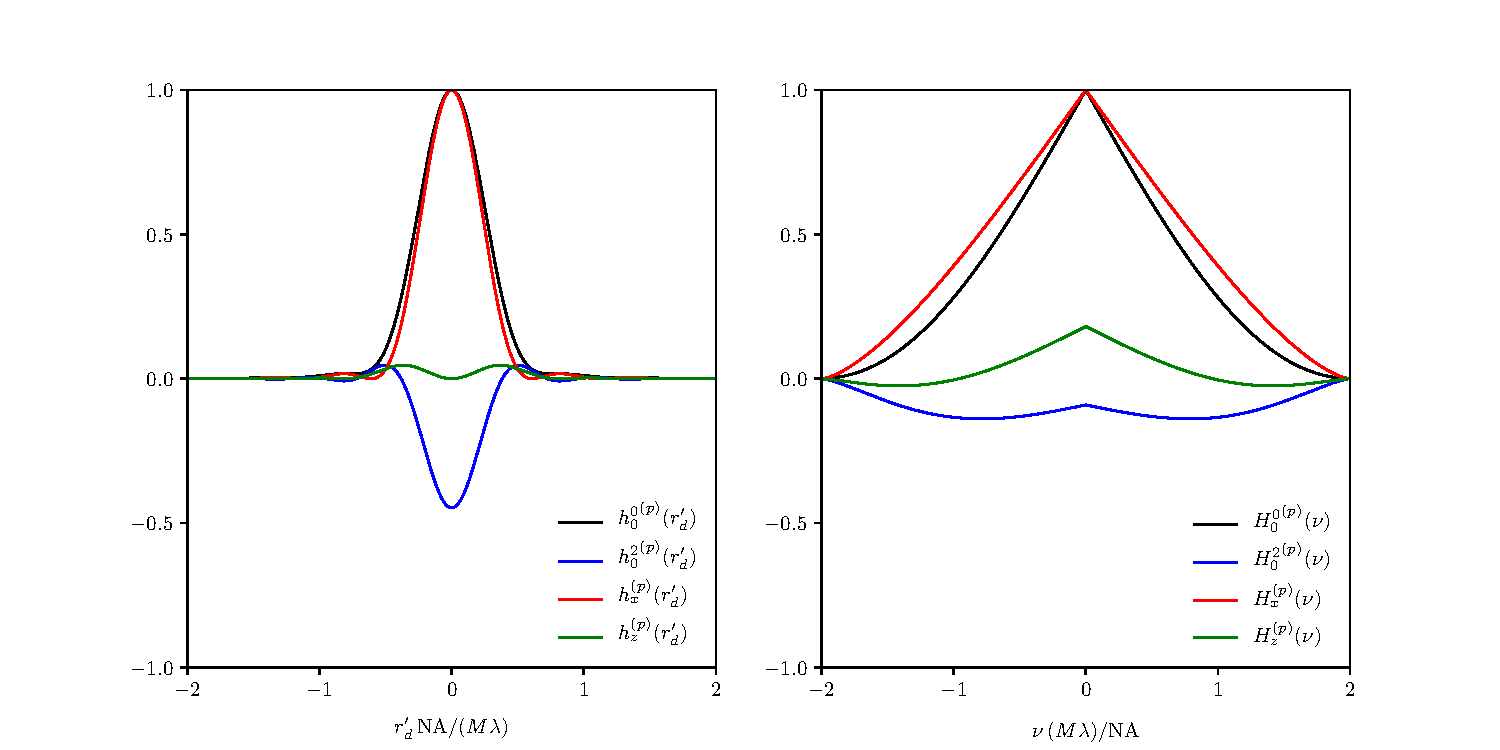
\includegraphics[width = 1.\textwidth]{../calculations/compare-ft/psfs.pdf}
   \caption{\textbf{Left:} Point spread functions and \textbf{Right:} optical
     transfer functions for a single-view fluorescence microscope with
     $\text{NA}=0.8$ and $n_o=1.33$ under the paraxial approximation.
     \textbf{Black:} $l=0, m=0$ spherical harmonic---an isotropic distribution
     of fluorophores. \textcolor{blue}{\textbf{Blue:}} $l=2, m=0$ spherical
     harmonic---negative fluorophores near the transverse plane, positive
     fluorophores near the optical axis. \textcolor{red}{\textbf{Red:}}
     $x$-oriented dipole. \textcolor{OliveGreen}{\textbf{Green:}} $z$-oriented
     dipole.}
   \label{fig:para}
\end{figure}
    
\bibliography{report}{}
\bibliographystyle{unsrt}

\appendix
\section{Products of real spherical harmonics}\label{realspherical}
The six products of $l=1$ spherical harmonics are
\begin{align}
y_1^{-1}y_1^{-1}\sqrt{\pi} &= \frac{1}{2 }y_0^0 - \frac{\sqrt{5}}{10 }y_2^0 - \frac{\sqrt{15}}{10 }y_2^2,\\ 
y_1^{-1}y_1^0\sqrt{\pi} &= \frac{\sqrt{15}}{10 }y_2^{-1} ,\\
y_1^{-1}y_1^1\sqrt{\pi} &= - \frac{\sqrt{15}}{10 }y_2^{-2} ,\\
y_1^0y_1^0\sqrt{\pi} &= \frac{1}{2 }y_0^0 + \frac{\sqrt{5}}{5 }y_2^0 ,\\
y_1^0y_1^1\sqrt{\pi} &= \frac{\sqrt{15}}{10 }y_2^1 ,\\
y_1^1y_1^1\sqrt{\pi} &= \frac{1}{2 }y_0^0 - \frac{\sqrt{5}}{10 }y_2^0 + \frac{\sqrt{15}}{10 }y_2^2.
\end{align}
The fifteen products of $l=2$ spherical harmonics are
\begin{align}
y_2^{-2}y_2^{-2}\sqrt{\pi} &= \frac{1}{2 }y_0^{0} - \frac{\sqrt{5}}{7 }y_2^{0} + \frac{1}{14 }y_4^{0} - \frac{\sqrt{35}}{14 }y_4^{4} \\
y_2^{-2}y_2^{-1}\sqrt{\pi} &= - \frac{\sqrt{15}}{14 }y_2^{1} + \frac{\sqrt{10}}{28 }y_4^{1} + \frac{\sqrt{70}}{28 }y_4^{3} \\
y_2^{-2}y_2^{0}\sqrt{\pi} &= - \frac{\sqrt{5}}{7 }y_2^{-2} + \frac{\sqrt{15}}{14 }y_4^{-2} \\
y_2^{-2}y_2^{1}\sqrt{\pi} &= - \frac{\sqrt{15}}{14 }y_2^{-1} - \frac{\sqrt{70}}{28 }y_4^{-3} + \frac{\sqrt{10}}{28 }y_4^{-1} \\
y_2^{-2}y_2^{2}\sqrt{\pi} &= \frac{\sqrt{35}}{14 }y_4^{-4} \\
y_2^{-1}y_2^{-1}\sqrt{\pi} &= \frac{1}{2 }y_0^{0} + \frac{\sqrt{5}}{14 }y_2^{0} - \frac{\sqrt{15}}{14 }y_2^{2} - \frac{2}{7 }y_4^{0} - \frac{\sqrt{5}}{7 }y_4^{2} \\
y_2^{-1}y_2^{0}\sqrt{\pi} &= \frac{\sqrt{5}}{14 }y_2^{-1} + \frac{\sqrt{30}}{14 }y_4^{-1} \\
y_2^{-1}y_2^{1}\sqrt{\pi} &= - \frac{\sqrt{15}}{14 }y_2^{-2} - \frac{\sqrt{5}}{7 }y_4^{-2} \\
y_2^{-1}y_2^{2}\sqrt{\pi} &= - \frac{\sqrt{15}}{14 }y_2^{-1} + \frac{\sqrt{70}}{28 }y_4^{-3} + \frac{\sqrt{10}}{28 }y_4^{-1} \\
y_2^{0}y_2^{0}\sqrt{\pi} &= \frac{1}{2 }y_0^{0} + \frac{\sqrt{5}}{7 }y_2^{0} + \frac{3}{7 }y_4^{0} \\
y_2^{0}y_2^{1}\sqrt{\pi} &= \frac{\sqrt{5}}{14 }y_2^{1} + \frac{\sqrt{30}}{14 }y_4^{1} \\
y_2^{0}y_2^{2}\sqrt{\pi} &= - \frac{\sqrt{5}}{7 }y_2^{2} + \frac{\sqrt{15}}{14 }y_4^{2} \\
y_2^{1}y_2^{1}\sqrt{\pi} &= \frac{1}{2 }y_0^{0} + \frac{\sqrt{5}}{14 }y_2^{0} + \frac{\sqrt{15}}{14 }y_2^{2} - \frac{2}{7 }y_4^{0} + \frac{\sqrt{5}}{7 }y_4^{2} \\
y_2^{1}y_2^{2}\sqrt{\pi} &= \frac{\sqrt{15}}{14 }y_2^{1} - \frac{\sqrt{10}}{28 }y_4^{1} + \frac{\sqrt{70}}{28 }y_4^{3} \\
y_2^{2}y_2^{2}\sqrt{\pi} &= \frac{1}{2 }y_0^{0} - \frac{\sqrt{5}}{7 }y_2^{0} + \frac{1}{14 }y_4^{0} + \frac{\sqrt{35}}{14 }y_4^{4}
\end{align}

\section{Paraxial coherent transfer function}\label{paraxialctf}
In this appendix we calculate the paraxial CTF for a single-view fluorescence
microscope. We start by plugging Eq. \ref{eq:paracsf} (the paraxial CSF) into Eq.
\ref{eq:csfdef2}
\begin{align}
  {\mb{E}_l^m}^{(p)}(\bs{\nu}) \propto \int_{\mathbb{S}^2}d\so{}\int_{\mathbb{R}^2}d\rd{}'\,
\begin{bmatrix}
    a^{(p)}(r_d')y_1^{1}(\so{}) + 2ib^{(p)}(r_d')\cos\phi_d'y_1^{0}(\so{})\\
    a^{(p)}(r_d')y_1^{-1}(\so{}) + 2ib^{(p)}(r_d')\sin\phi_d'y_1^{0}(\so{})\\
    0\\
  \end{bmatrix}
  y_l^m(\so{})\thinspace\me^{-i 2\pi\rd{}'\cdot\bs{\nu}}. 
\end{align}
We split the integral into two parts by writing
\begin{align}
  {\mb{E}_l^m}^{(p)}(\bs{\nu}) &\propto \int_{\mathbb{S}^2}d\so{}\, \mb{E}^{(p)}(\bs{\nu};\so{}) y_l^m(\so{}),\\ \label{eq:splitup}
  \mb{E}^{(p)}(\bs{\nu};\so{}) &\equiv  \int_{\mathbb{R}^2}d\rd{}'\
\begin{bmatrix}
    a^{(p)}(r_d')y_1^{1}(\so{}) + 2ib^{(p)}(r_d')\cos\phi_d'y_1^{0}(\so{})\\
    a^{(p)}(r_d')y_1^{-1}(\so{}) + 2ib^{(p)}(r_d')\sin\phi_d'y_1^{0}(\so{})\\
    0\\
  \end{bmatrix}
  \thinspace\me^{-i 2\pi\rd{}'\cdot\bs{\nu}}. 
\end{align}
Substituting $a^{(p)}(r_d')$ and $b^{(p)}(r_d')$ using Eq. \ref{eq:abparadef} gives
\begin{align}
  \mb{E}^{(p)}(\bs{\nu}; \so{}) = \int_{\mathbb{R}^2}d\rd{}'\,
\begin{bmatrix}
    \frac{J_1(2\pi \nu_or_d')}{\pi \nu_or_d'}y_1^m(\so{}) + 2i\frac{\text{NA}}{n_o}\left[\frac{J_2(2\pi \nu_or_d')}{\pi \nu_or_d'}\right]\cos\phi_d'y_1^0(\so{})\\
    \frac{J_1(2\pi \nu_or_d')}{\pi \nu_or_d'}y_1^{-1}(\so{}) + 2i\frac{\text{NA}}{n_o}\left[\frac{J_2(2\pi ar_d')}{\pi \nu_or_d'}\right]\sin\phi_d'y_1^0(\so{})\\
    0\\
  \end{bmatrix}
  \thinspace\me^{-i 2\pi\rd{}'\cdot\bs{\nu}}.
\end{align}
We can rewrite this in terms of three two-dimensional Fourier transforms
\begin{align}
  \mb{E}^{(p)}(\bs{\nu}; \so{}) \propto 
\begin{bmatrix}
    t_1(\bs{\nu})y_1^1(\so{}) + t_2(\bs{\nu})y_1^0(\so{})\\
    t_1(\bs{\nu})y_1^{-1}(\so{}) + t_3(\bs{\nu})y_1^0(\so{})\\
    0\\
  \end{bmatrix}\label{eq:tint}
\end{align}
where
\begin{align}
  t_1(\bs{\nu}) &\equiv \frac{1}{\pi \nu_o}\int_{\mathbb{R}^2}d\rd{}'\,  \frac{J_1(2\pi \nu_or_d')}{r_d'}\, \me^{-i 2\pi\rd{}'\cdot\bs{\nu}},\\
  t_2(\bs{\nu}) &\equiv \frac{2i}{\pi \nu_o}\frac{\text{NA}}{n_o}\int_{\mathbb{R}^2}d\rd{}'\, \frac{J_2(2\pi \nu_or_d')}{r_d'}\cos\phi_d'\, \me^{-i 2\pi\rd{}'\cdot\bs{\nu}},\\
  t_3(\bs{\nu}) &\equiv \frac{2i}{\pi \nu_o}\frac{\text{NA}}{n_o}\int_{\mathbb{R}^2}d\rd{}'\, \frac{J_2(2\pi \nu_or_d')}{r_d'}\sin\phi_d'\, \me^{-i 2\pi\rd{}'\cdot\bs{\nu}}.
\end{align}
All three of the functions to be transformed are separable in polar coordinates,
so we can rewrite the Fourier transform as a sum of weighted Hankel transforms
\cite{goodman1996}. In general, if a function $g(r, \theta)$ is separable in
polar coordinates then we can rewrite it as
$g(r, \theta) = g_{R}(r)g_{\Theta}(\theta)$ and its two-dimensional Fourier transform
is given by
\begin{align}
  \mathcal{F}\{g(r, \theta)\} = \sum_{k=-\infty}^{\infty}c_k(-i)^k\me^{ik\phi}\mathcal{H}_k\{g_R(r)\}
\end{align}
where
\begin{align}
  c_k = \frac{1}{2\pi}\int_0^{2\pi}d\theta\, g_{\Theta}(\theta)\me^{-ik\theta}
\end{align}
and $\mathcal{H}_k\{\}$ is the Hankel transform of order $k$ given by
\begin{align}
  \mathcal{H}_k\{g_R(r)\} = 2\pi\int_0^{\infty}dr\, r g_R(r)J_k(2\pi r \nu).
\end{align}
First, we evaluate $t_1(\bs{\nu})$. The Fourier transform will be in polar
coordinates, so we define polar coordinates in frequency space as
$\bs{\nu} \equiv \nu\cos\phi_\nu\mh{x} + \nu\sin\phi_\nu\mh{y} \equiv \nu_x\mh{x} + \nu_y\mh{y}$. The
angular part of $J_z(\nu_or_d')/r_d'$ is a constant, so $c_k = \delta(k)$ which
means we only need to evaluate the zero-order Hankel transform
\begin{align}
  t_1(\bs{\nu}) = \frac{1}{\pi \nu_o}\mathcal{H}_0\left\{\frac{J_1(2\pi \nu_or_d')}{r_d'}\right\}.
\end{align}
From tabulated Hankel transforms we find that
\begin{align}
  \mathcal{H}_{\mu}\left\{\frac{J_{\mu+1}(2\pi \nu_or_d')}{r_d'}\right\} =
  \frac{1}{2\pi}\nu_o^{-\mu-1}\nu^\mu\, \Pi\left(\frac{\nu}{a}\right)\label{eq:hankstar}
\end{align}
when $\nu_o > 0$ and $\text{Re}(\mu) > -\frac{3}{2}$ \cite{poul1998}. Applying this result
we find that
\begin{align}
  t_1(\bs{\nu}) =
    \frac{1}{2\pi^2 \nu_o^{2}}\, \Pi\left(\frac{\nu}{\nu_o}\right)\label{eq:t1final}.
\end{align}
To evaluate $t_2(\bs{\nu})$ and $t_3(\bs{\nu})$ we need to be careful with the angular part. For $t_2(\bs{\nu})$
the angular part of the function is $\cos\phi_d' = \frac{1}{2}\left(e^{i\phi_d'} + e^{-i\phi_d'}\right)$. Therefore, $c_k = \frac{1}{2}\delta(k-1) + \frac{1}{2}\delta(k+1)$ and we have to evaluate two Hankel transforms given by
\begin{align}
  t_2(\bs{\nu}) = \frac{2i}{\pi \nu_o}\frac{\text{NA}}{n_o}\left[ie^{-i\phi_{\nu}}\mathcal{H}_{-1}\left\{\frac{J_2(2\pi \nu_or_d')}{\pi \nu_or_d'}\right\} - ie^{i\phi_{\nu}}\mathcal{H}_{1}\left\{\frac{J_2(2\pi \nu_or_d')}{\pi ar_d'}\right\}\right].
\end{align}
To put the Hankel transforms in the form of Eq. \ref{eq:hankstar} we apply
$\mathcal{H}_\mu = (-1)^\mu\mathcal{H}_{-\mu}$ to get
\begin{align}
  t_2(\bs{\nu}) = \frac{2i}{\pi \nu_o}\frac{\text{NA}}{n_o}\left[-ie^{-i\phi_{\nu}}\mathcal{H}_{1}\left\{\frac{J_2(2\pi \nu_or_d')}{\pi \nu_or_d'}\right\} - ie^{i\phi_{\nu}}\mathcal{H}_{1}\left\{\frac{J_2(2\pi \nu_or_d')}{\pi \nu_or_d'}\right\}\right].
\end{align}
Applying Eq. \ref{eq:hankstar} and simplifying gives
\begin{align}
  t_2(\bs{\nu}) =
    \frac{1}{\pi^2 \nu_o^3}\frac{\text{NA}}{n_o}\nu(e^{-i\phi_\nu} + e^{i\phi_\nu})\, \Pi\left(\frac{\nu}{\nu_o}\right)
\end{align}
Finally, 
\begin{align}
  t_2(\bs{\nu}) =
    \frac{1}{\pi^2 \nu_o^3}\frac{\text{NA}}{n_o}\nu\cos\phi_{\nu}\, \Pi\left(\frac{\nu}{a}\right)\label{eq:t2final}
\end{align}
Similarly, 
\begin{align}
  t_3(\bs{\nu}) =
    \frac{1}{\pi^2 \nu_o^3}\frac{\text{NA}}{n_o}\nu\sin\phi_{\nu}\, \Pi\left(\frac{\nu}{a}\right)\label{eq:t3final}
\end{align}
Plugging Eqs. \ref{eq:t1final}, \ref{eq:t2final}, and \ref{eq:t3final} into Eq.
\ref{eq:tint} and normalizing gives
\begin{align}
  {\mb{E}}^{(p)}(\bs{\nu}; \so{}) =
\begin{bmatrix}
  y_1^1(\so{}) + \frac{2}{\nu_o}\frac{\text{NA}}{n_o}\nu\cos\phi_\nu y_1^0(\so{})\\
  y_1^{-1}(\so{}) + \frac{2}{\nu_o}\frac{\text{NA}}{n_o}\nu\sin\phi_\nu y_1^0(\so{})\\
  0\\
  \end{bmatrix}\, \Pi\left(\frac{\nu}{\nu_o}\right). \label{eq:paractfsp}
\end{align}
Finally, we find the paraxial CTF by evaluating the angular integral in Eq.
\ref{eq:splitup} 
\begin{align}
  {\mb{E}_l^m}^{(p)}(\bs{\nu}) =
\begin{bmatrix}
  \delta(l-1, m-1) + \frac{2}{\nu_o}\frac{\text{NA}}{n_o}\nu\cos\phi_\nu\delta(l-1, m)\\
  \delta(l-1, m+1) + \frac{2}{\nu_o}\frac{\text{NA}}{n_o}\nu\sin\phi_\nu\delta(l-1, m)\\
  0\\
  \end{bmatrix}\, \Pi\left(\frac{\nu}{\nu_o}\right).
\end{align}

% \section{Paraxial optical transfer function}\label{paraxialotf}
% In this appendix we calculate the paraxial OTF for a single-view fluorescence
% microscope. We start with Eq. \ref{eq:otfdef2}
% \begin{align}
%   H_l^m(\bs{\nu}) \propto \int_{\mathbb{S}^2}d\so{}\int_{\mathbb{R}^2}d\rd{}'\, h(\rd{}', \so{}) y_l^m(\so{})\thinspace\me^{-i 2\pi \rd{}'\cdot\bs{\nu}}.
% \end{align}
% We could plug in the paraxial PSF and evaluate the integrals, but this will lead
% us to Fourier transforms that cannot be found in tables. Instead we use a trick
% from scalar Fourier optics and write the OTF in terms of the detected electric
% field \cite{goodman1996}
% \begin{align}
%   H_l^m(\bs{\nu}) \propto \int_{\mathbb{S}^2}d\so{}\int_{\mathbb{R}^2}d\rd{}'\, \left|\mb{e}_d(\rd{}', \so{})\right|^2 y_l^m(\so{})\thinspace\me^{-i 2\pi \rd{}'\cdot\bs{\nu}}.
% \end{align}
% Next, we manipulate this equation to
% \begin{align}
%   H_l^m(\bs{\nu}) &\propto \int_{\mathbb{S}^2}d\so{}\, y_l^m(\so{})\int_{\mathbb{R}^2}d\rd{}'\, \mb{e}^{\dagger}_d(\rd{}', \so{})\mb{e}_d(\rd{}', \so{})\, \me^{-i 2\pi \rd{}'\cdot\bs{\nu}},\\
%   H_l^m(\bs{\nu}) &\propto \int_{\mathbb{S}^2}d\so{}\, y_l^m(\so{})\int_{\mathbb{R}^2}d\rd{}'\, \int_{\mathbb{R}^2}d\rd{}''\, \mb{e}^{\dagger}_d(\rd{}', \so{})\mb{e}_d(\rd{}'', \so{})\delta(\rd{}'' - \rd{}')\, \me^{-i 2\pi \rd{}''\cdot\bs{\nu}},\\
%   H_l^m(\bs{\nu}) &\propto \int_{\mathbb{S}^2}d\so{}\, y_l^m(\so{})\int_{\mathbb{R}^2}d\bs{\tau}\,\int_{\mathbb{R}^2}d\rd{}'\, \int_{\mathbb{R}^2}d\rd{}''\, \mb{e}^{\dagger}_d(\rd{}', \so{})\mb{e}_d(\rd{}'', \so{})\me^{-i 2\pi\bs{\tau}(\rd{}'' - \rd{}')}\me^{-i 2\pi \rd{}''\cdot\bs{\nu}},\\
%   H_l^m(\bs{\nu}) &\propto \int_{\mathbb{S}^2}d\so{}\, y_l^m(\so{})\int_{\mathbb{R}^2}d\bs{\tau}\,\left[\int_{\mathbb{R}^2}d\rd{}'\, \mb{e}^{\dagger}_d(\rd{}', \so{}) \me^{i 2\pi\rd{}'\cdot \bs{\tau}}\right]\left[\int_{\mathbb{R}^2}d\rd{}''\, \mb{e}_d(\rd{}'', \so{})\me^{-i 2\pi \rd{}''\cdot(\bs{\nu} + \bs{\tau})}\right],\\
%   H_l^m(\bs{\nu}) &\propto \int_{\mathbb{S}^2}d\so{}\, y_l^m(\so{})\int_{\mathbb{R}^2}d\bs{\tau}\,\mb{E}^{\dagger}(\bs{\tau}; \so{})\mb{E}(\bs{\tau} + \bs{\nu}; \so{}). \label{eq:hlmauto}
% \end{align}
% We have followed the proof for the Wiener-Kinchin theorem \cite{papoulis2002, wiener} to explicitly show how the angular integral affects the usual scalar
% calculation. Eq. \ref{eq:hlmauto} shows that we can calculate the OTF by taking
% the vector autocorrelation of the spatial CTF then projecting the result onto
% the spherical harmonics.

% We will rewrite Eq. \ref{eq:hlmauto} in two parts
% \begin{align}
%   H_l^m(\bs{\nu}) &\propto \int_{\mathbb{S}^2}d\so{}\, y_l^m(\so{}) H(\bs{\nu}; \so{})  \label{eq:hlmauto2}\\
%   H(\bs{\nu}; \so{}) &\equiv \int_{\mathbb{R}^2}d\bs{\tau}\,\mb{E}^{\dagger}(\bs{\tau}- \bs{\nu}/2; \so{})\mb{E}(\bs{\tau} + \bs{\nu}/2; \so{}). \label{eq:hlmspatial}
% \end{align}
% Notice the change of variable to simplify the autocorrelation. In the previous
% section we calculated the CTF in the paraxial case as 
% \begin{align}
%   {\mb{E}}^{(p)}(\bs{\nu}; \so{}) =
% \begin{bmatrix}
%   y_1^1(\so{}) + \frac{2}{\nu_o}\frac{\text{NA}}{n_o}\nu\cos\phi_\nu y_1^0(\so{})\\
%   y_1^{-1}(\so{}) + \frac{2}{\nu_o}\frac{\text{NA}}{n_o}\nu\sin\phi_\nu y_1^0(\so{})\\
%   0\\
%   \end{bmatrix}\, \Pi\left(\frac{\nu}{\nu_o}\right). \label{eq:ctfparax}
% \end{align}
% By introducing $\bs{\tau} \equiv \tau_x\mh{x} + \tau_y\mh{y} \equiv \tau\cos\phi_\tau\mh{x} + \tau\sin\phi_\tau\mh{y}$
% we can plug Eq. \ref{eq:ctfparax} into Eq. \ref{eq:hlmspatial} and find that
% \begin{align}
%     H^{(p)}(\bs{\nu}; \so{}) \propto \int_{\mathbb{R}^2}d\bs{\tau}\, &\begin{bmatrix}
%   y_1^1(\so{}) + \frac{2}{\nu_o}\frac{\text{NA}}{n_o}(\tau_x - \frac{1}{2}\nu_x) y_1^0(\so{})\\
%   y_1^{-1}(\so{}) + \frac{2}{\nu_o}\frac{\text{NA}}{n_o}(\tau_y - \frac{1}{2}\nu_y) y_1^0(\so{})\\
%   0\\
% \end{bmatrix}^{\dagger}
%   \begin{bmatrix}
%   y_1^1(\so{}) + \frac{2}{\nu_o}\frac{\text{NA}}{n_o}(\tau_x + \frac{1}{2}\nu_x) y_1^0(\so{})\\
%   y_1^{-1}(\so{}) + \frac{2}{\nu_o}\frac{\text{NA}}{n_o}(\tau_y + \frac{1}{2}\nu_y) y_1^0(\so{})\\
%   0\\
% \end{bmatrix}\nonumber \\
%   &\Pi\left(\frac{\tau - \nu/2}{\nu_o}\right)\Pi\left(\frac{\tau + \nu/2}{\nu_o}\right).
% \end{align}
% Expanding the inner product gives
% \begin{align}
%     H^{(p)}(\bs{\nu}; \so{}) \propto \int_{\mathbb{R}^2}d\bs{\tau}\, &
%       \{y_1^1(\so{})\}^2  + \left\{\frac{2}{\nu_o}\frac{\text{NA}}{n_o}y_1^0(\so{})\right\}^2(\tau_x - \frac{1}{2}\nu_x)(\tau_x + \frac{1}{2}\nu_x) + \nonumber \\
%                                                                  &\{y_1^{-1}(\so{})\}^2 + \left\{\frac{2}{\nu_o}\frac{\text{NA}}{n_o}y_1^0(\so{})\right\}^2(\tau_y - \frac{1}{2}\nu_y)(\tau_y + \frac{1}{2}\nu_y) + \nonumber \\
%                                                                  &\left\{\frac{2}{\nu_o}\frac{\text{NA}}{n_o}y_1^0(\so{})y_1^1(\so{})\right\}(\tau_x - \frac{1}{2}\nu_x) + \left\{\frac{2}{\nu_o}\frac{\text{NA}}{n_o}y_1^0(\so{})y_1^1(\so{})\right\}(\tau_x + \frac{1}{2}\nu_x) \nonumber \\
%   &\left\{\frac{2}{\nu_o}\frac{\text{NA}}{n_o}y_1^0(\so{})y_1^{-1}(\so{})\right\}(\tau_y - \frac{1}{2}\nu_y) + \left\{\frac{2}{\nu_o}\frac{\text{NA}}{n_o}y_1^0(\so{})y_1^{-1}(\so{})\right\}(\tau_y + \frac{1}{2}\nu_y) \nonumber \\  
% &\Pi\left(\frac{\tau - \nu/2}{\nu_o}\right)\Pi\left(\frac{\tau + \nu/2}{\nu_o}\right). 
% \end{align}
% All of the terms with a single $(\tau_\cdot \pm \frac{1}{2}\nu_\cdot)$ term are
% correlations of an odd function with an even function, so they are zero.
% Therefore
% \begin{align}
%     H^{(p)}(\bs{\nu}; \so{}) \propto \int_{\mathbb{R}^2}d\bs{\tau}\, &
%       \{y_1^1(\so{})\}^2  + \left\{\frac{2}{\nu_o}\frac{\text{NA}}{n_o}y_1^0(\so{})\right\}^2(\tau_x - \frac{1}{2}\nu_x)(\tau_x + \frac{1}{2}\nu_x) + \nonumber \\
%                                                                  &\{y_1^{-1}(\so{})\}^2 + \left\{\frac{2}{\nu_o}\frac{\text{NA}}{n_o}y_1^0(\so{})\right\}^2(\tau_y - \frac{1}{2}\nu_y)(\tau_y + \frac{1}{2}\nu_y) + \nonumber \\
% &\Pi\left(\frac{\tau - \nu/2}{\nu_o}\right)\Pi\left(\frac{\tau + \nu/2}{\nu_o}\right). 
% \end{align}
% After expanding the spherical harmonics we can rewrite this equation in terms of
% two autocorrelations
% \begin{align}
%     H^{(p)}(\nu; \so{}) &\propto \Big[A^{(p)}(\nu) + 2B^{(p)}(\nu)\Big]y_0^0(\so{}) + \frac{1}{\sqrt{5}}\Big[-A^{(p)}(\nu) + 4B^{(p)}(\nu)\Big]y_2^0(\so{})\label{eq:hinter}
% \end{align}
% where
% \begin{align}
%   A^{(p)}(\nu) &\equiv \frac{1}{\pi\nu_o^2}\int_{\mathbb{R}^2}d\bs{\tau}\, \Pi\left(\frac{\tau - \nu/2}{\nu_o}\right)\Pi\left(\frac{\tau + \nu/2}{\nu_o}\right),\\
%   B^{(p)}(\nu) &\equiv \frac{\text{NA}^2}{\pi\nu_o^4n_o^2} \int_{\mathbb{R}^2}d\bs{\tau}\, \left[(\tau_x - \nu_x/2)(\tau_x + \nu_x/2) + (\tau_y - \nu_y/2)(\tau_y + \nu_y/2)\right]\nonumber \\ &\hspace{17em}\Pi\left(\frac{\tau - \nu/2}{\nu_o}\right)\Pi\left(\frac{\tau + \nu/2}{\nu_o}\right).
% \end{align}
% I've used the constant $\frac{1}{\pi\nu_o^2}$ in front of both autocorrelations
% so that the results are normalized, but these constants are not essential. Also,
% notice that both autocorrelations are rotationally symmetric, so we can write
% them as a function of $\nu$ instead of $\bs{\nu}$. We can evaluate these
% integrals with the help of the geometric construction shown in Figure
% \ref{fig:geometry} \cite{goodman1996}.

% \begin{figure}[h]
%  \captionsetup{width=1.0\linewidth}
%  \centering
%    \centering
%    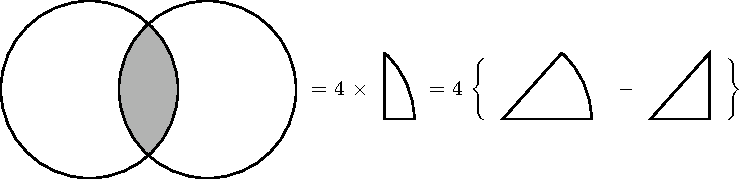
\includegraphics[width = 0.8\textwidth]{../figures/geometry/geometry.pdf}
%    \caption{Geometric construction for evaluating $A^{(p)}(\bs{\nu})$ and
%      $B^{(p)}(\bs{\nu})$. We need to find the boundaries of integration for the
%      overlapping region of two circles with radius $\nu_o$ and distance $\nu$
%      between their centers. The region is given by four times the difference in
%      area between a sector of angle $\arccos\left(\frac{\nu}{2\nu_o}\right)$ and
%      a triangle with base $\nu/2$ and hypotenuse $\nu_o$.}
%    \label{fig:geometry}
% \end{figure}

% Starting with $A^{(p)}(\nu)$ we find that
% \begin{align}
%   A^{(p)}(\nu) &= \frac{4}{\pi\nu_o^2}\left[\left(\int\limits_0^{\nu_o} d\tau\, \tau\int\limits_0^{\arccos\left(\frac{\nu}{2\nu_o}\right)}d\phi_{\tau}\right) - \left(\int\limits_0^{\nu/2}d\tau_x \int\limits_0^{\tau_x\frac{2\nu_o}{\nu}\sqrt{1 - \left(\frac{\nu}{2\nu_o}\right)^2}}d\tau_y\right)\right]\Pi\left(\frac{\nu}{2\nu_o}\right)\\
%   A^{(p)}(\nu) &= \frac{4}{\pi\nu_o^2}\left[\left(\int\limits_0^{\nu_o} d\tau\,\tau\arccos\left(\frac{\nu}{2\nu_o}\right)\right) - \left(\int\limits_0^{\nu/2}d\tau_x \tau_x \frac{2\nu_o}{\nu}\sqrt{1 - \left(\frac{\nu}{2\nu_o}\right)^2}\right)\right]\Pi\left(\frac{\nu}{2\nu_o}\right)\\
%   A^{(p)}(\nu) &= \frac{2}{\pi}\left[\arccos\left(\frac{\nu}{2\nu_o}\right) - \frac{\nu}{2\nu_o}\sqrt{1 - \left(\frac{\nu}{2\nu_o}\right)^2}\right]\Pi\left(\frac{\nu}{2\nu_o}\right).
% \end{align}
% Notice that $A^{(p)}(\nu)$ is the normalized OTF for fluorescence
% microscope with isotropic samples under the paraxial and scalar approximations.
% Next we evaluate $B^{(p)}(\nu)$ using the same geometric construction. This
% integral is rotationally symmetric, so we start by rewriting it as 
% \begin{align}
%   B^{(p)}(\nu) =  \frac{4\text{NA}^2}{\pi\nu_o^4n_o^2}\Bigg[\int\limits_0^{\nu_o} d\tau\, \tau \int\limits_0^{\arccos\left(\frac{\nu}{2\nu_o}\right)}d\phi_{\tau}(-\tau^2\cos^2\phi_{\tau} + \nu\tau\cos\phi_{\tau}) - \int\limits_0^{\nu/2}d\tau_x \int\limits_0^{\tau_x \frac{2\nu_o}{\nu}\sqrt{1 - \left(\frac{\nu}{2\nu_o}\right)^2}}d\tau_y(-\tau_x^2 + \nu\tau_x)\Bigg]\Pi\left(\frac{\nu}{2\nu_o}\right).\\
% \end{align}
% For the first inner integral we make use of
% \begin{align}
%   \int\limits_0^{\arccos(z)} d\phi \cos^2\phi &= \frac{1}{2}z\sqrt{1 - z^2} + \frac{1}{2}\arccos(z), \\
%   \int\limits_0^{\arccos(z)} d\phi \cos\phi &= \sqrt{1 - z^2}.
% \end{align}
% This results in
% \begin{align}
%   B^{(p)}(\nu)&=\frac{4\text{NA}^2}{\pi\nu_o^4n_o^2}\Bigg[\int\limits_0^{\nu_o} d\tau\, \frac{-\tau^3}{2}\left(\frac{\nu}{2\nu_o}\sqrt{1 - \left(\frac{\nu}{2\nu_o}\right)^2} + \arccos\left(\frac{\nu}{2a}\right)\right) + \nu\tau^2\sqrt{1 - \left(\frac{\nu}{2\nu_o}\right)}\nonumber \\ &\hspace{5em}- \int\limits_0^{\nu/2}d\tau_x \left(-\tau_x^3 + \nu\tau_x^2\right)\frac{2 \nu_o}{\nu}\sqrt{1 - \left(\frac{\nu}{2\nu_o}\right)^2}\Bigg]\Pi\left(\frac{\nu}{2\nu_o}\right),\\
%   B^{(p)}(\nu) &=  \frac{4\text{NA}^2}{\pi\nu_o^4n_o^2}\Bigg[\frac{-\nu_o^4}{8}\left(\frac{\nu}{2\nu_o}\sqrt{1 - \left(\frac{\nu}{2\nu_o}\right)^2} + \arccos\left(\frac{\nu}{2\nu_o}\right) \right) + \frac{2\nu_o^4}{3}\frac{\nu}{2\nu_o}\sqrt{1 - \left(\frac{\nu}{2\nu_o}\right)}\nonumber \\ &\hspace{5em} - \frac{5\nu^2\nu_o^2}{48}\frac{\nu}{2\nu_o}\sqrt{1 - \left(\frac{\nu}{2\nu_o}\right)^2}\Bigg]\Pi\left(\frac{\nu}{2\nu_o}\right),\\
%   B^{(p)}(\nu) &=  \frac{\text{NA}^2}{2\pi n_o^2}\Bigg[\left(\frac{-\nu}{2\nu_o}\sqrt{1 - \left(\frac{\nu}{2\nu_o}\right)^2} - \arccos\left(\frac{\nu}{2\nu_o}\right) \right) + \frac{16}{3}\frac{\nu}{2\nu_o}\sqrt{1 - \left(\frac{\nu}{2\nu_o}\right)}\nonumber \\ &\hspace{5em} - \frac{5\nu^2}{6\nu_o^2}\frac{\nu}{2\nu_o}\sqrt{1 - \left(\frac{\nu}{2\nu_o}\right)^2}\Bigg]\Pi\left(\frac{\nu}{2\nu_o}\right),\\
%   B^{(p)}(\nu) &= \frac{\text{NA}^2}{2\pi n_o^2}\left[-\arccos\left(\frac{\nu}{2\nu_o}\right) + \left(\frac{13}{3} - \frac{5\nu^2}{6\nu_o^2}\right)\frac{\nu}{2\nu_o} \sqrt{1 - \left(\frac{\nu}{2\nu_o}\right)^2}\right]\Pi\left(\frac{\nu}{2\nu_o}\right),\\
%   B^{(p)}(\nu) &= \frac{2}{\pi}\left(\frac{2\text{NA}}{n_o}\right)^2\left[-\arccos\left(\frac{\nu}{2\nu_o}\right) + \frac{1}{3}\left[13 - 10\left(\frac{\nu}{2\nu_o}\right)^2\right]\frac{\nu}{2\nu_o} \sqrt{1 - \left(\frac{\nu}{2\nu_o}\right)^2}\right]\Pi\left(\frac{\nu}{2\nu_o}\right).                 
% \end{align}

% Now that we've evaluated the autocorrelations we can complete the OTF
% calculation. By plugging Eq. \ref{eq:hinter} into Eq. \ref{eq:hlmauto2},
% performing the angular integral, and normalizing, we get the complete
% spatio-angular transfer function
% \begin{align}
%   {H_l^m}^{(p)}(\nu) &= {H_0^0}^{(p)}(\nu)\delta(l, m) + {H_2^0}^{(p)}(\nu)\delta(l-2, m),\\
%   {H_0^0}^{(p)}(\nu) &\equiv \frac{A^{(p)}(\nu) + 2B^{(p)}(\nu)}{1 + 8(\text{NA}/n_o)^2},\\
%   {H_2^0}^{(p)}(\nu) &\equiv \frac{-A^{(p)}(\nu) + 4B^{(p)}}{\sqrt{5}\, [1 + 8(\text{NA}/n_o)^2]}.
% \end{align}
% where
% \begin{align}
%   {A}^{(p)}(\nu) &= \frac{2}{\pi}\left[\arccos\left(\frac{\nu}{2\nu_o}\right) - \frac{\nu}{2\nu_o}\sqrt{1 - \left(\frac{\nu}{2\nu_o}\right)^2}\right]\Pi\left(\frac{\nu}{2\nu_o}\right),\\
%   B^{(p)}(\nu) &= \frac{2}{\pi}\left(\frac{2\text{NA}}{n_o}\right)^2\left[-\arccos\left(\frac{\nu}{2\nu_o}\right) + \frac{1}{3}\left[13 - 10\left(\frac{\nu}{2\nu_o}\right)^2\right]\frac{\nu}{2\nu_o} \sqrt{1 - \left(\frac{\nu}{2\nu_o}\right)^2}\right]\Pi\left(\frac{\nu}{2\nu_o}\right).                 
% \end{align}

\section{Paraxial optical transfer function}\label{paraxialotf2}    
In this appendix we calculate the paraxial OTF for a single-view fluorescence
microscope. We start with Eq. \ref{eq:otfdef2}
\begin{align}
  {H_l^m}^{(p)}(\bs{\nu}) \propto \int_{\mathbb{S}^2}d\so{}\int_{\mathbb{R}^2}d\rd{}'\, h^{(p)}(\rd{}', \so{}) y_l^m(\so{})\thinspace\me^{-i 2\pi \rd{}'\cdot\bs{\nu}}.
  \label{eq:appotf}
\end{align}
where the paraxial PSF is given by Eq. \ref{eq:concisepsf}
\begin{align}
  h^{(p)}(\rd{}', \so{}) &= {h_0^0}^{(p)}(\rd{}')y_0^0(\so{}) + {h_2^0}^{(p)}(\rd{}')y_2^0(\so{}),\\ \label{eq:parapsf}
  {h_0^0}^{(p)}(\rd{}') &\equiv {a^{(p)}}^2(r_d') + 2{b^{(p)}}^2(r_d'),\\
  {h_2^0}^{(p)}(\rd{}') &\equiv \frac{1}{\sqrt{5}}\left[- {a^{(p)}}^2(r_d') + 4{b^{(p)}}^2(r_d')\right]. 
\end{align}
Plugging Eq. \ref{eq:parapsf} into Eq. \ref{eq:appotf} and evaluating the
angular integral gives
\begin{align}
  {H_l^m}^{(p)}(\bs{\nu}) \propto \int_{\mathbb{R}^2}d\rd{}'\, \left[{h_0^0}^{(p)}(\rd{}')\delta(l, m) + {h_2^0}^{(p)}(\rd{}')\delta(l-2, m)\right] \me^{-i 2\pi \rd{}'\cdot\bs{\nu}}. \label{eq:appotf2}
\end{align}
Using the operator notation $\mathcal{F}_2\{f(\mb{r})\} = \int_{\mathbb{R}^2}d\mb{r}\{f(\mb{r})\}\me^{-i 2\pi \mb{r}\cdot\bs{\nu}}$, we can rewrite Eq. \ref{eq:appotf2} as 
\begin{align}
  {H_l^m}^{(p)}(\bs{\nu}) &\propto \mathcal{F}_2\{{h_0^0}^{(p)}(\rd{}')\delta(l, m) + {h_2^0}^{(p)}(\rd{}')\delta(l-2, m) \},\\
  {H_l^m}^{(p)}(\bs{\nu}) &\propto \left[\mathcal{F}_2\left\{{a^{(p)}}^2(r_d')\right\} + 2\mathcal{F}_2\left\{{b^{(p)}}^2(r_d')\right\}\right]\delta(l, m) + \\&\hspace{1em}\left[-\mathcal{F}_2\left\{{a^{(p)}}^2(r_d')\right\} + 4\mathcal{F}_2\left\{{b^{(p)}}^2(r_d')\right\}\right]\delta(l-2, m).
\end{align}
To calculate $\mathcal{F}_2\left\{{a^{(p)}}^2(r_d')\right\}$ we can use the
autocorrelation theorem \cite{goodman1996}
p\begin{align}
  \mathcal{F}_2\left\{f^2(r)\right\} = \mathcal{F}_2\left\{f(r)\right\} \star_2 \mathcal{F}\left\{f(r)\right\},
\end{align}
where $\star_2$ denotes a two-dimensional autocorrelation. We can rewrite
$\mathcal{F}_2\left\{{a^{(p)}}^2(r_d')\right\}$ as
\begin{align}
  \mathcal{F}_2\left\{{a^{(p)}}^2(r_d')\right\} &= \mathcal{F}_2\left\{\frac{J_1(2\pi\nu_o r_d')}{\pi\nu_o r_d'}\right\} \star_2 \mathcal{F}_2\left\{\frac{J_1(2\pi\nu_o r_d')}{\pi\nu_o r_d'}\right\}.
\end{align}
Next, we notice that the two-dimensional Fourier transform is radially
symmetric, so it can be written as a zero-order Hankel transform
\begin{align}
\mathcal{F}_2\left\{{a^{(p)}}^2(r_d')\right\} &= \mathcal{H}_0\left\{\frac{J_1(2\pi\nu_o r_d')}{\pi\nu_o r_d'}\right\} \star_2 \mathcal{H}_0\left\{\frac{J_1(2\pi\nu_o r_d')}{\pi\nu_o r_d'}\right\}, 
\end{align}
where the $k$-order Hankel transform is defined as
\begin{align}
  \mathcal{H}_k\left\{f(r)\right\} = 2\pi \int_0^\infty dr\, r f(r)J_k(2\pi r\nu).
\end{align}
Finally, we can apply the following Hankel transform identity
\begin{align}
  \mathcal{H}_{k}\left\{\frac{J_{k+1}(2\pi \nu_or_d')}{\pi\nu_o r_d'}\right\} =
  \frac{2\nu^k}{\nu_o^{k+1}}\, \Pi\left(\frac{\nu}{\nu_o}\right)\label{eq:hankstar2},
\end{align}
when $\nu_o > 0$ and $\text{Re}(k) > -\frac{3}{2}$ \cite{poul1998} which gives
\begin{align}
  \mathcal{F}_2\left\{{a^{(p)}}^2(r_d')\right\} &= \left[\frac{2}{\nu_o}\Pi\left(\frac{\nu}{\nu_o}\right)\right] \star_2 \left[\frac{2}{\nu_o}\Pi\left(\frac{\nu}{\nu_o}\right)\right],\\
  \mathcal{F}_2\left\{{a^{(p)}}^2(r_d')\right\} &= \frac{4}{\nu_o^2}\left[\Pi\left(\frac{\nu}{\nu_o}\right)\right] \star_2 \left[\Pi\left(\frac{\nu}{\nu_o}\right)\right].
\end{align}
The autocorrelation is a geometry problem of finding the area of overlap of two
displaced circles. Using the geometric construction in Fig. \ref{fig:geometry} we find that
\begin{figure}[h]
 \captionsetup{width=1.0\linewidth}
 \centering
   \centering
   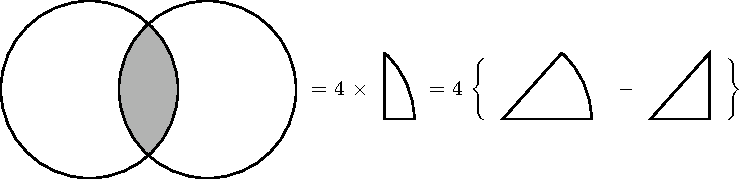
\includegraphics[width = 0.8\textwidth]{../figures/geometry/geometry.pdf}
   \caption{Geometric construction for evaluating the autocorrelations. We need
     to integrate over the overlapping region of two circles with radius $\nu_o$
     and distance $\nu$ between their centers. The region is given by four times
     the difference in area between a sector of angle
     $\arccos\left(\frac{\nu}{2\nu_o}\right)$ and a triangle with base $\nu/2$
     and hypotenuse $\nu_o$.}
   \label{fig:geometry}
\end{figure}
\begin{align}
  \mathcal{F}_2\left\{{a^{(p)}}^2(r_d')\right\}&= \frac{16}{\nu_o^2}\left[\left(\int\limits_0^{\nu_o} d\tau\, \tau\int\limits_0^{\arccos\left(\frac{\nu}{2\nu_o}\right)}d\phi_{\tau}\right) - \left(\int\limits_0^{\nu/2}d\tau_x \int\limits_0^{\tau_x\frac{2\nu_o}{\nu}\sqrt{1 - \left(\frac{\nu}{2\nu_o}\right)^2}}d\tau_y\right)\right]\Pi\left(\frac{\nu}{2\nu_o}\right),\\
  \mathcal{F}_2\left\{{a^{(p)}}^2(r_d')\right\} &= \frac{16}{\nu_o^2}\left[\left(\int\limits_0^{\nu_o} d\tau\,\tau\arccos\left(\frac{\nu}{2\nu_o}\right)\right) - \left(\int\limits_0^{\nu/2}d\tau_x \tau_x \frac{2\nu_o}{\nu}\sqrt{1 - \left(\frac{\nu}{2\nu_o}\right)^2}\right)\right]\Pi\left(\frac{\nu}{2\nu_o}\right),\\
  \mathcal{F}_2\left\{{a^{(p)}}^2(r_d')\right\} &= 8\left[\arccos\left(\frac{\nu}{2\nu_o}\right) - \frac{\nu}{2\nu_o}\sqrt{1 - \left(\frac{\nu}{2\nu_o}\right)^2}\right]\Pi\left(\frac{\nu}{2\nu_o}\right).
\end{align}

Next, we calculate $\mathcal{F}_2\left\{{b^{(p)}}^2(r_d')\right\}$. If we follow
the same steps as we did for $\mathcal{F}_2\left\{{a^{(p)}}^2(r_d')\right\}$, we
will reach a dead end because there is no Hankel transform identity that we can
use. Instead, we rewrite $\mathcal{F}_2\left\{{b^{(p)}}^2(r_d')\right\}$ in the
following way so that we can use the Hankel transform identity in Eq. \ref{eq:hankstar2}
\begin{align}
  \mathcal{F}_2\left\{{b^{(p)}}^2(r_d')\right\} = \mathcal{F}_2\left\{{b^{(p)}}^2(r_d')\cos^2(\phi_d')\right\} + \mathcal{F}_2\left\{{b^{(p)}}^2(r_d')\cos^2(\phi_d')\right\}.
\end{align}
Now we apply the autocorrelation theorem
\begin{align}
  \mathcal{F}_2\left\{{b^{(p)}}^2(r_d')\right\} = \left[\mathcal{F}_2\left\{{b^{(p)}}(r_d')\cos(\phi_d')\right\} \star_2 \mathcal{F}_2\left\{{b^{(p)}}(r_d')\cos(\phi_d')\right\}\right] + \left[\mathcal{F}_2\left\{{b^{(p)}}(r_d')\sin(\phi_d')\right\} \star_2 \mathcal{F}_2\left\{{b^{(p)}}(r_d')\sin(\phi_d')\right\}\right]. \label{eq:int3}
\end{align}
The two autocorrelated Fourier transforms are separable in polar coordinates, so
they can be expanded in terms of Hankel transforms \cite{goodman1996}. In
general, if a function $f(r, \theta)$ is separable in polar coordinates then we
can rewrite it as $f(r, \theta) = f_{R}(r)f_{\Theta}(\theta)$ and its
two-dimensional Fourier transform can be expanded in terms of Hankel transforms
using
\begin{align}
  \mathcal{F}\{f(r, \theta)\} = \sum_{k=-\infty}^{\infty}c_k(-i)^k\me^{ik\phi}\mathcal{H}_k\{f_R(r)\},
\end{align}
where
\begin{align}
  c_k = \frac{1}{2\pi}\int_0^{2\pi}d\theta\, f_{\Theta}(\theta)\me^{-ik\theta}. 
\end{align}
Applying the Hankel transform expansion to $\mathcal{F}_2\left\{{b^{(p)}}(r_d')\cos(\phi_d')\right\}$ gives
\begin{align}
  \mathcal{F}_2\left\{{b^{(p)}}(r_d')\cos(\phi_d')\right\} = \frac{1}{2}\left[i\me^{i\phi_\nu}\mathcal{H}_{-1}\{{b^{(p)}}(r_d')\} - i\me^{-i\phi_\nu}\mathcal{H}_{1}\{{b^{(p)}}(r_d')\}\right].
\end{align}
Next, we apply the identity $\mathcal{H}_\mu = (-1)^\mu\mathcal{H}_{-\mu}$ and simplify
\begin{align}
  \mathcal{F}_2\left\{{b^{(p)}}(r_d')\cos(\phi_d')\right\} = -i\cos\phi_\nu \mathcal{H}_{1}\{{b^{(p)}}(r_d')\}.
\end{align}
Next, we evaluate the Hankel transform using Eq. \ref{eq:hankstar2}
\begin{align}
  \mathcal{H}_{1}\{{b^{(p)}}(r_d')\} = \mathcal{H}_{1}\left\{\frac{J_{2}(2\pi \nu_or_d')}{\pi\nu_o r_d'}\right\} =
  \left(\frac{\text{NA}}{n_o}\right)\frac{2\nu}{\nu_o^{2}}\, \Pi\left(\frac{\nu}{\nu_o}\right).
\end{align}
Therefore, 
\begin{align}
  \mathcal{F}_2\left\{{b^{(p)}}(r_d')\cos(\phi_d')\right\} = -\left(\frac{\text{NA}}{n_o}\right)\frac{2i\nu\cos\phi_\nu}{\nu_o^2}\, \Pi\left(\frac{\nu}{\nu_o}\right) = -\left(\frac{\text{NA}}{n_o}\right)\frac{2i\nu_x}{\nu_o^2}\, \Pi\left(\frac{\nu}{\nu_o}\right).
\end{align}
Similarly,
\begin{align}
  \mathcal{F}_2\left\{{b^{(p)}}(r_d')\sin(\phi_d')\right\} = -\left(\frac{\text{NA}}{n_o}\right)\frac{2i\nu\sin\phi_\nu}{\nu_o^2}\, \Pi\left(\frac{\nu}{\nu_o}\right) = -\left(\frac{\text{NA}}{n_o}\right)\frac{2i\nu_y}{\nu_o^2}\, \Pi\left(\frac{\nu}{\nu_o}\right).  
\end{align}
Now we can plug these back in to the autocorrelation in Eq. \ref{eq:int3}
\begin{align}
    \mathcal{F}_2\left\{{b^{(p)}}^2(r_d')\right\} &= -\left(\frac{\text{NA}}{n_o}\right)^2\frac{4}{\nu_0^4}\left\{\left[\nu_x\, \Pi\left(\frac{\nu}{\nu_o}\right)\right] \star_2 \left[\nu_x\, \Pi\left(\frac{\nu}{\nu_o}\right)\right]\right\} - \left(\frac{\text{NA}}{n_o}\right)^2\frac{4}{\nu_0^4}\left\{\left[\nu_y\, \Pi\left(\frac{\nu}{\nu_o}\right)\right] \star_2 \left[\nu_y\, \Pi\left(\frac{\nu}{\nu_o}\right)\right]\right\}.\label{eq:auto}
\end{align}
These autocorrelations can be evaluated by finding the weighted area of overlap
of two circles. Neither of the autocorrelations is radially symmetric, but we
know that their sum must be radially symmetric because ${b^{(p)}}^2(r_d')$ is
radially symmetric. We recognize that the first autocorrelation is largest for
shifts along the $x$ axis and smallest for shifts along the $y$ axis with a
smooth $\cos^2\phi_\nu$ weighting between the two extremes. The same is true for
the second autocorrelation except with the $x$ and $y$ axes exchanged and a
$\sin^2\phi_\nu$ weighting between the two extremes. Therefore, the sum of the two
autocorrelations can be rewritten as the sum of either autocorrelation shifted along
the $x$ axis and the $y$ axis
\begin{align}
    \mathcal{F}_2\left\{{b^{(p)}}^2(r_d')\right\} &= -\left(\frac{\text{NA}}{n_o}\right)^2\frac{4}{\nu_0^4}\left\{\left[\nu_x\, \Pi\left(\frac{\nu}{\nu_o}\right)\right] \star_2^x \left[\nu_x\, \Pi\left(\frac{\nu}{\nu_o}\right)\right]\right\} - \left(\frac{\text{NA}}{n_o}\right)^2\frac{4}{\nu_0^4}\left\{\left[\nu_x\, \Pi\left(\frac{\nu}{\nu_o}\right)\right] \star_2^y \left[\nu_x\, \Pi\left(\frac{\nu}{\nu_o}\right)\right]\right\}.
\end{align}
where $\star_2^x$ denotes a two-dimensional autocorrelation for shifts along the
$x$ axis.

We can use the same limits of integration as we did previously, but we need to
include a weighted integrand. First, we evaluate the autocorrelation for shifts
along the $x$-axis
\begin{align}
  &\frac{-4}{\nu_0^4}\left\{\left[\nu_x\, \Pi\left(\frac{\nu}{\nu_o}\right)\right] \star_2^x \left[\nu_x\, \Pi\left(\frac{\nu}{\nu_o}\right)\right]\right\} = \\
  &=  \frac{-16}{\nu_o^4}\Bigg[\int\limits_0^{\nu_o} d\tau\, \tau \int\limits_0^{\arccos\left(\frac{\nu}{2\nu_o}\right)}d\phi_{\tau}(-\tau^2\cos^2\phi_{\tau} + \nu\tau\cos\phi_{\tau}) - \int\limits_0^{\nu/2}d\tau_x \int\limits_0^{\tau_x \frac{2\nu_o}{\nu}\sqrt{1 - \left(\frac{\nu}{2\nu_o}\right)^2}}d\tau_y(-\tau_x^2 + \nu\tau_x)\Bigg]\Pi\left(\frac{\nu}{2\nu_o}\right).
\end{align}
For the first inner integral we make use of
\begin{align}
  \int\limits_0^{\arccos(z)} d\phi \cos^2\phi &= \frac{1}{2}z\sqrt{1 - z^2} + \frac{1}{2}\arccos(z), \\
  \int\limits_0^{\arccos(z)} d\phi \cos\phi &= \sqrt{1 - z^2}.
\end{align}
This results in
\begin{align}
  &=\frac{-16}{\nu_o^4}\Bigg[\int\limits_0^{\nu_o} d\tau\, \frac{-\tau^3}{2}\left(\frac{\nu}{2\nu_o}\sqrt{1 - \left(\frac{\nu}{2\nu_o}\right)^2} + \arccos\left(\frac{\nu}{2a}\right)\right) + \nu\tau^2\sqrt{1 - \left(\frac{\nu}{2\nu_o}\right)}\nonumber \\ &\hspace{5em}- \int\limits_0^{\nu/2}d\tau_x \left(-\tau_x^3 + \nu\tau_x^2\right)\frac{2 \nu_o}{\nu}\sqrt{1 - \left(\frac{\nu}{2\nu_o}\right)^2}\Bigg]\Pi\left(\frac{\nu}{2\nu_o}\right),\\
  &=  \frac{-16}{\nu_o^4}\Bigg[\frac{-\nu_o^4}{8}\left(\frac{\nu}{2\nu_o}\sqrt{1 - \left(\frac{\nu}{2\nu_o}\right)^2} + \arccos\left(\frac{\nu}{2\nu_o}\right) \right) + \frac{2\nu_o^4}{3}\frac{\nu}{2\nu_o}\sqrt{1 - \left(\frac{\nu}{2\nu_o}\right)}\nonumber \\ &\hspace{5em} - \frac{5\nu^2\nu_o^2}{48}\frac{\nu}{2\nu_o}\sqrt{1 - \left(\frac{\nu}{2\nu_o}\right)^2}\Bigg]\Pi\left(\frac{\nu}{2\nu_o}\right),\\
  &=  2\Bigg[\left(\frac{\nu}{2\nu_o}\sqrt{1 - \left(\frac{\nu}{2\nu_o}\right)^2} + \arccos\left(\frac{\nu}{2\nu_o}\right) \right) - \frac{16}{3}\frac{\nu}{2\nu_o}\sqrt{1 - \left(\frac{\nu}{2\nu_o}\right)}\nonumber \\ &\hspace{5em} + \frac{5\nu^2}{6\nu_o^2}\frac{\nu}{2\nu_o}\sqrt{1 - \left(\frac{\nu}{2\nu_o}\right)^2}\Bigg]\Pi\left(\frac{\nu}{2\nu_o}\right),\\
  &= 2\left[\arccos\left(\frac{\nu}{2\nu_o}\right) - \left(\frac{13}{3} - \frac{5\nu^2}{6\nu_o^2}\right)\frac{\nu}{2\nu_o} \sqrt{1 - \left(\frac{\nu}{2\nu_o}\right)^2}\right]\Pi\left(\frac{\nu}{2\nu_o}\right),\\
  &= \left[2\arccos\left(\frac{\nu}{2\nu_o}\right) - \frac{2}{3}\left[13 - 10\left(\frac{\nu}{2\nu_o}\right)^2\right]\frac{\nu}{2\nu_o} \sqrt{1 - \left(\frac{\nu}{2\nu_o}\right)^2}\right]\Pi\left(\frac{\nu}{2\nu_o}\right).\label{eq:auto1}
\end{align}
Next, we evaluate the autocorrelation for shifts along the $y$-axis
\begin{align}
  &\frac{-4}{\nu_0^4}\left\{\left[\nu_x\, \Pi\left(\frac{\nu}{\nu_o}\right)\right] \star_2^y \left[\nu_x\, \Pi\left(\frac{\nu}{\nu_o}\right)\right]\right\} = \\
  &=  \frac{-16}{\nu_o^4}\Bigg[\int\limits_0^{\nu_o} d\tau\, \tau \int\limits_0^{\arccos\left(\frac{\nu}{2\nu_o}\right)}d\phi_{\tau}(-\tau^2\sin^2\phi_{\tau}) - \int\limits_0^{\nu/2}d\tau_x \int\limits_0^{\tau_x \frac{2\nu_o}{\nu}\sqrt{1 - \left(\frac{\nu}{2\nu_o}\right)^2}}d\tau_y(-\tau_y^2)\Bigg]\Pi\left(\frac{\nu}{2\nu_o}\right).
\end{align}
For the first inner integral we make use of
\begin{align}
  \int\limits_0^{\arccos(z)} d\phi \sin^2\phi &= -\frac{1}{2}z\sqrt{1 - z^2} + \frac{1}{2}\arccos(z).
\end{align}
This results in
\begin{align}
  &=\frac{-16}{\nu_o^4}\Bigg[\int\limits_0^{\nu_o} d\tau\, \frac{-\tau^3}{2}\left(\frac{-\nu}{2\nu_o}\sqrt{1 - \left(\frac{\nu}{2\nu_o}\right)^2} + \arccos\left(\frac{\nu}{2a}\right)\right) - \int\limits_0^{\nu/2}d\tau_x \frac{-\tau_x^3}{3}\left(\frac{2 \nu_o}{\nu}\sqrt{1 - \left(\frac{\nu}{2\nu_o}\right)^2}\right)^3\Bigg]\Pi\left(\frac{\nu}{2\nu_o}\right),\\
  &=  \frac{-16}{\nu_o^4}\Bigg[\frac{-\nu_o^4}{8}\left(\frac{-\nu}{2\nu_o}\sqrt{1 - \left(\frac{\nu}{2\nu_o}\right)^2} + \arccos\left(\frac{\nu}{2\nu_o}\right) \right) + \frac{\nu_o^4}{12}\frac{\nu}{2\nu_o}\sqrt[3]{1 - \left(\frac{\nu}{2\nu_o}\right)^2}\Bigg]\Pi\left(\frac{\nu}{2\nu_o}\right),\\
  &=  \Bigg[2\arccos\left(\frac{\nu}{2\nu_o}\right) - 2\frac{\nu}{2\nu_o}\sqrt{1 - \left(\frac{\nu}{2\nu_o}\right)^2} - \frac{4}{3}\frac{\nu}{2\nu_o}\sqrt[3]{1 - \left(\frac{\nu}{2\nu_o}\right)^2}\Bigg]\Pi\left(\frac{\nu}{2\nu_o}\right). \label{eq:auto2}
\end{align}
Combining the results in Eqs. \ref{eq:auto1} and \ref{eq:auto2} gives us the final Fourier transform
\begin{align}
  \mathcal{F}_2\left\{{b^{(p)}}^2(r_d')\right\} &= 4\left(\frac{\text{NA}}{n_o}\right)^2\left[\arccos\left(\frac{\nu}{2\nu_o}\right) - \frac{1}{3}\left[8 - 5\left(\frac{\nu}{2\nu_o}\right)^2\right]\frac{\nu}{2\nu_o} \sqrt{1 - \left(\frac{\nu}{2\nu_o}\right)^2} - \frac{1}{3}\frac{\nu}{2\nu_o}\sqrt[3]{1 - \left(\frac{\nu}{2\nu_o}\right)^2}\right]\Pi\left(\frac{\nu}{2\nu_o}\right),\\
    \mathcal{F}_2\left\{{b^{(p)}}^2(r_d')\right\} &= 4\left(\frac{\text{NA}}{n_o}\right)^2\left[\arccos\left(\frac{\nu}{2\nu_o}\right) - \left[3 - 2\left(\frac{\nu}{2\nu_o}\right)^2\right]\frac{\nu}{2\nu_o} \sqrt{1 - \left(\frac{\nu}{2\nu_o}\right)^2}\right]\Pi\left(\frac{\nu}{2\nu_o}\right).
\end{align}
Now that we've evaluated $\mathcal{F}_2\left\{{a^{(p)}}^2(r_d')\right\}$ and $\mathcal{F}_2\left\{{b^{(p)}}^2(r_d')\right\}$, we can plug the results into the following equation and we have the complete spatio-angular transfer function
\begin{align}
  {H_l^m}^{(p)}(\bs{\nu}) &\propto \left[\mathcal{F}_2\left\{{a^{(p)}}^2(r_d')\right\} + 2\mathcal{F}_2\left\{{b^{(p)}}^2(r_d')\right\}\right]\delta(l, m) + \\&\hspace{1em}\left[-\mathcal{F}_2\left\{{a^{(p)}}^2(r_d')\right\} + 4\mathcal{F}_2\left\{{b^{(p)}}^2(r_d')\right\}\right]\delta(l-2, m).
\end{align}
After refactoring and normalizing, we have the final spatio-angular transfer function
\begin{align}
  {H_l^m}^{(p)}(\nu) &= {H_0^0}^{(p)}(\nu)\delta(l, m) + {H_2^0}^{(p)}(\nu)\delta(l-2, m),\\
  {H_0^0}^{(p)}(\nu) &\equiv \frac{A^{(p)}(\nu) + 2B^{(p)}(\nu)}{1 + (\text{NA}/n_o)^2},\\
  {H_2^0}^{(p)}(\nu) &\equiv \frac{-A^{(p)}(\nu) + 4B^{(p)}}{\sqrt{5}\, [1 + (\text{NA}/n_o)^2]},
\end{align}
where
\begin{align}
  {A}^{(p)}(\nu) &= \frac{2}{\pi}\left[\arccos\left(\frac{\nu}{2\nu_o}\right) - \frac{\nu}{2\nu_o}\sqrt{1 - \left(\frac{\nu}{2\nu_o}\right)^2}\right]\Pi\left(\frac{\nu}{2\nu_o}\right),\\
  B^{(p)}(\nu) &= \frac{1}{\pi}\left(\frac{\text{NA}}{n_o}\right)^2\left[\arccos\left(\frac{\nu}{2\nu_o}\right) - \left[3 - 2\left(\frac{\nu}{2\nu_o}\right)^2\right]\frac{\nu}{2\nu_o} \sqrt{1 - \left(\frac{\nu}{2\nu_o}\right)^2}\right]\Pi\left(\frac{\nu}{2\nu_o}\right).                 
\end{align}

\tikzstyle{block} = [draw, fill=white, rectangle, 
    minimum height=2cm, minimum width=3.5cm, text width=3cm, align=center]
\tikzstyle{sum} = [draw, fill=white, circle, node distance=4cm]
\tikzstyle{input} = [coordinate]
\tikzstyle{output} = [coordinate]
\tikzstyle{pinstyle} = [pin edge={to-,thin,black}]
\begin{figure}
\begin{tikzpicture}[auto, node distance=3cm,>=latex]
    \node [input, name=input] {};
    \node [block, align=center] (csf) {CSF\\ $\tilde{\mb{e}}_d(\rd{} - M\ro{}, \so{})$};
    \node [block,  right of=csf, node distance=6cm] (ctf) {CTF\\ $\mb{E}_l^m(\bs{\nu})$};
    \node [block, below of=ctf, node distance=4cm] (otf) {OTF\\ $H_l^m(\bs{\nu})$};
    \node [block, below of=csf, node distance=4cm] (psf) {PSF\\ $h(\rd{} - M\ro{}, \so{})$};
    
    \draw [<->] (csf) -- node[name=u, text width=3cm, align=center] {Tube Lens\\ $\mathcal{F}_{\mathbb{R}^2}$} (ctf);        
    \draw [->] (ctf) -- node[name=v, right] {$\mathcal{F}_{\mathbb{S}^2}[\mb{E}_l^m(\bs{\nu})\star_{\mathbb{R}^2} \mb{E}_l^m(\bs{\nu})]$} (otf);
    \draw [<->] (psf) -- node[below] {$\mathcal{F}_{\mathbb{R}^3\times\mathbb{S}^2}$} (otf);
    \draw [->] (csf) -- node[name=v, text width=4cm, align=center, left] {Detector\\ $|\mb{\tilde{e}}_d(\rd{} - M\ro{}, \so{})|^2_{\mathbb{R}^2}$} (psf);
      \end{tikzpicture}
      \centering
      \captionsetup{width=1.0\linewidth}
      \caption{Summary of relationships between the CSF, CTF, PSF, and OTF where
        $\mathcal{F}_D$, $|\cdot|_D$, and $\star_D$ denote the Fourier
        transform, norm, and autocorrelation over the set $D$, respectively. See
        \cite{goodman1996} and \cite{mertz2009} for analogous diagrams under
        scalar optics approximations.}
    \end{figure}

\end{document}
